% ******************************* PhD Thesis Template **************************
% Please have a look at the README.md file for info on how to use the template

\documentclass[a4paper,12pt,times,authoryear,print,index,custombib]{Classes/PhDThesisPSnPDF}

% ******************************************************************************
% ******************************* Class Options ********************************
% *********************** See README for more details **************************
% ******************************************************************************

% `a4paper'(The University of Cambridge PhD thesis guidelines recommends a page
% size a4 - default option) or `a5paper': A5 Paper size is also allowed as per
% the Cambridge University Engineering Deparment guidelines for PhD thesis
%
% `11pt' or `12pt'(default): Font Size 10pt is NOT recommended by the University
% guidelines
%
% `oneside' or `twoside'(default): Printing double side (twoside) or single
% side.
%
% `print': Use `print' for print version with appropriate margins and page
% layout. Leaving the options field blank will activate Online version.
%
% `index': For index at the end of the thesis
%
% `draftclassic': For draft mode without loading any images (same as draft in book)
%
% `draft': Special draft mode with line numbers, images, and water mark with
% timestamp and custom text. Position of the text can also be modified.
%
% `abstract': To generate only the title page and abstract page with
% dissertation title and name, to submit to the Student Registry
%
% `chapter`: This option enables only the specified chapter and it's references
%  Useful for review and corrections.
%
% ************************* Custom Page Margins ********************************
%
% `custommargin`: Use `custommargin' in options to activate custom page margins,
% which can be defined in the preamble.tex. Custom margin will override
% print/online margin setup.
%
% *********************** Choosing the Fonts in Class Options ******************
%
% `times' : Times font with math support. (The Cambridge University guidelines
% recommend using times)
%
% `fourier': Utopia Font with Fourier Math font (Font has to be installed)
%            It's a free font.
%
% `customfont': Use `customfont' option in the document class and load the
% package in the preamble.tex
%
% default or leave empty: `Latin Modern' font will be loaded.
%
% ********************** Choosing the Bibliography style ***********************
%
% `authoryear': For author-year citation eg., Krishna (2013)
%
% `numbered': (Default Option) For numbered and sorted citation e.g., [1,5,2]
%
% `custombib': Define your own bibliography style in the `preamble.tex' file.
%              `\RequirePackage[square, sort, numbers, authoryear]{natbib}'.
%              This can be also used to load biblatex instead of natbib
%              (See Preamble)
%
% **************************** Choosing the Page Style *************************
%
% `default (leave empty)': For Page Numbers in Header (Left Even, Right Odd) and
% Chapter Name in Header (Right Even) and Section Name (Left Odd). Blank Footer.
%
% `PageStyleI': Chapter Name next & Page Number on Even Side (Left Even).
% Section Name & Page Number in Header on Odd Side (Right Odd). Footer is empty.
%
% `PageStyleII': Chapter Name on Even Side (Left Even) in Header. Section Number
% and Section Name in Header on Odd Side (Right Odd). Page numbering in footer

% Uncomment to change page style
%\pagestyle{PageStyleII}

% ********************************** Preamble **********************************
% Preamble: Contains packages and user-defined commands and settings
% ******************************************************************************
% ****************************** Custom Margin *********************************

% Add `custommargin' in the document class options to use this section
% Set {innerside margin / outerside margin / topmargin / bottom margin}  and
% other page dimensions
\ifsetCustomMargin
  \RequirePackage[left=37mm,right=30mm,top=35mm,bottom=30mm]{geometry}
  \setFancyHdr % To apply fancy header after geometry package is loaded
\fi

% Add spaces between paragraphs
%\setlength{\parskip}{0.5em}
% Ragged bottom avoids extra whitespaces between paragraphs
\raggedbottom
% To remove the excess top spacing for enumeration, list and description
%\usepackage{enumitem}
%\setlist[enumerate,itemize,description]{topsep=0em}

% *****************************************************************************
% ******************* Fonts (like different typewriter fonts etc.)*************

% Add `customfont' in the document class option to use this section

\ifsetCustomFont
  % Set your custom font here and use `customfont' in options. Leave empty to
  % load computer modern font (default LaTeX font).
  %\RequirePackage{helvet}

  % For use with XeLaTeX
  %  \setmainfont[
  %    Path              = ./libertine/opentype/,
  %    Extension         = .otf,
  %    UprightFont = LinLibertine_R,
  %    BoldFont = LinLibertine_RZ, % Linux Libertine O Regular Semibold
  %    ItalicFont = LinLibertine_RI,
  %    BoldItalicFont = LinLibertine_RZI, % Linux Libertine O Regular Semibold Italic
  %  ]
  %  {libertine}
  %  % load font from system font
  %  \newfontfamily\libertinesystemfont{Linux Libertine O}
\fi

% *****************************************************************************
% **************************** Custom Packages ********************************

% ************************* Algorithms and Pseudocode **************************

%\usepackage{algpseudocode}


% ********************Captions and Hyperreferencing / URL **********************

% Captions: This makes captions of figures use a boldfaced small font.
%\RequirePackage[small,bf]{caption}

\RequirePackage[labelsep=space,tableposition=top]{caption}
\renewcommand{\figurename}{Fig.} %to support older versions of captions.sty


% *************************** Graphics and figures *****************************

%\usepackage{rotating}
%\usepackage{wrapfig}

% Uncomment the following two lines to force Latex to place the figure.
% Use [H] when including graphics. Note 'H' instead of 'h'
%\usepackage{float}
%\restylefloat{figure}

% Subcaption package is also available in the sty folder you can use that by
% uncommenting the following line
% This is for people stuck with older versions of texlive
%\usepackage{sty/caption/subcaption}
\usepackage{subcaption}

% ********************************** Tables ************************************
\usepackage{booktabs} % For professional looking tables
\usepackage{multirow}

%\usepackage{multicol}
%\usepackage{longtable}
%\usepackage{tabularx}


% *********************************** SI Units *********************************
\usepackage{siunitx} % use this package module for SI units


% ******************************* Line Spacing *********************************

% Choose linespacing as appropriate. Default is one-half line spacing as per the
% University guidelines

\doublespacing
% \onehalfspacing
% \singlespacing


% ************************ Formatting / Footnote *******************************

% Don't break enumeration (etc.) across pages in an ugly manner (default 10000)
%\clubpenalty=500
%\widowpenalty=500

%\usepackage[perpage]{footmisc} %Range of footnote options


% *****************************************************************************
% *************************** Bibliography  and References ********************

%\usepackage{cleveref} %Referencing without need to explicitly state fig /table

% Add `custombib' in the document class option to use this section
\ifuseCustomBib
 %\RequirePackage[authoryear]{natbib} % CustomBib

% If you would like to use biblatex for your reference management, as opposed to the default `natbibpackage` pass the option `custombib` in the document class. Comment out the previous line to make sure you don't load the natbib package. Uncomment the following lines and specify the location of references.bib file

\RequirePackage[backend=biber, style=numeric-comp, citestyle=authoryear, sorting=ynt, natbib=true]{biblatex}
\addbibresource{References/references.bib} %Location of references.bib only for biblatex, Do not omit the .bib extension from the filename.

\fi

% changes the default name `Bibliography` -> `References'
\renewcommand{\bibname}{References}


% ******************************************************************************
% ************************* User Defined Commands ******************************
% ******************************************************************************

% *********** To change the name of Table of Contents / LOF and LOT ************

%\renewcommand{\contentsname}{My Table of Contents}
%\renewcommand{\listfigurename}{My List of Figures}
%\renewcommand{\listtablename}{My List of Tables}


% ********************** TOC depth and numbering depth *************************

\setcounter{secnumdepth}{2}
\setcounter{tocdepth}{2}


% ******************************* Nomenclature *********************************

% To change the name of the Nomenclature section, uncomment the following line

%\renewcommand{\nomname}{Symbols}


% ********************************* Appendix ***********************************

% The default value of both \appendixtocname and \appendixpagename is `Appendices'. These names can all be changed via:

%\renewcommand{\appendixtocname}{List of appendices}
%\renewcommand{\appendixname}{Appndx}

% *********************** Configure Draft Mode **********************************

% Uncomment to disable figures in `draft'
%\setkeys{Gin}{draft=true}  % set draft to false to enable figures in `draft'

% These options are active only during the draft mode
% Default text is "Draft"
%\SetDraftText{DRAFT}

% Default Watermark location is top. Location (top/bottom)
%\SetDraftWMPosition{bottom}

% Draft Version - default is v1.0
%\SetDraftVersion{v1.1}

% Draft Text grayscale value (should be between 0-black and 1-white)
% Default value is 0.75
%\SetDraftGrayScale{0.8}


% ******************************** Todo Notes **********************************
%% Uncomment the following lines to have todonotes.

%\ifsetDraft
%	\usepackage[colorinlistoftodos]{todonotes}
%	\newcommand{\mynote}[1]{\todo[author=kc391,size=\small,inline,color=green!40]{#1}}
%\else
%	\newcommand{\mynote}[1]{}
%	\newcommand{\listoftodos}{}
%\fi

% Example todo: \mynote{Hey! I have a note}

% *****************************************************************************
% ******************* Better enumeration my MB*************
\usepackage{enumitem}

\usepackage{times}
\usepackage{url}
\usepackage{latexsym}
\usepackage{amsmath}
\usepackage{amssymb}
\usepackage{breqn}
\usepackage{booktabs}
\usepackage{pbox}
\usepackage{multirow}
\usepackage{graphicx}
\usepackage{tablefootnote}
\usepackage{wrapfig}
\usepackage{epigraph}
\setlength{\epigraphwidth}{.5\textwidth}
\usepackage[official]{eurosym}
\usepackage{hyperref}
\hypersetup{citecolor=Brown}
\usepackage{setspace}

% ************************ Thesis Information & Meta-data **********************
% Thesis title and author information, refernce file for biblatex
% ************************ Thesis Information & Meta-data **********************
%% The title of the thesis
\title{Deep Generative Models of Text}
%\texorpdfstring is used for PDF metadata. Usage:
%\texorpdfstring{LaTeX_Version}{PDF Version (non-latex)} eg.,
%\texorpdfstring{$sigma$}{sigma}

%% Subtitle (Optional)
%\subtitle{Using the CUED template}

%% The full name of the author
\author{Kris Cao}

%% Department (eg. Department of Engineering, Maths, Physics)
\dept{Department of Computer Science}

%% University and Crest
\university{University of Cambridge}
% Crest minimum should be 30mm.
\crest{
\includegraphics[width=0.2\textwidth]{University_Crest}}
%% Use this crest, if you are using the college crest
%% Crest long miminum should be 65mm
%\crest{
\includegraphics[width=0.45\textwidth]{University_Crest_Long}}

%% College shield [optional] 
% Crest minimum should be 30mm.
%\collegeshield{\includegraphics[width=0.2\textwidth]{CollegeShields/Clare}}


%% Supervisor (optional)
%% for multiple supervisors, append each supervisor with the \newline command
%\supervisor{Prof. A.B. Supervisor\newline
%Prof. C.D. Supervisor}

%% Supervisor Role (optional) - Supervisor (default) or advisor
% \supervisorrole{\textbf{Supervisors: }}
%% if no title is desired:
% \supervisorrole{}

%% Supervisor line width: required to align supervisors
%\supervisorlinewidth{0.35\textwidth}

%% Advisor (optional)
%% for multiple advisors, append each advisor with the \newline command
%\advisor{Dr. A. Advisor\newline
%Dr. B. Advisor}
     
%% Advisor Role (optional) - Advisor (default) or leave empty
% \advisorrole{Advisors: }
%% if no title is required
% \advisorrole{}

%% Advisor line width: required to align supervisors
%\advisorlinewidth{0.25\textwidth}


%% You can redefine the submission text:
% Default as per the University guidelines:
% ``This dissertation is submitted for the degree of''
%\renewcommand{\submissiontext}{change the default text here if needed}

%% Full title of the Degree
\degreetitle{Doctor of Philosophy}

%% College affiliation (optional)
\college{Clare College}

%% Submission date
% Default is set as {\monthname[\the\month]\space\the\year}
\degreedate{October 2018}

% ***************************** Abstract Separate ******************************
% To printout only the titlepage and the abstract with the PhD title and the
% author name for submission to the Student Registry, use the `abstract' option in
% the document class.

\ifdefineAbstract
 \pagestyle{empty}
 \includeonly{Declaration/declaration, Abstract/abstract}
\fi

% ***************************** Chapter Mode ***********************************
% The chapter mode allows user to only print particular chapters with references
% Title, Contents, Frontmatter are disabled by default
% Useful option to review a particular chapter or to send it to supervisior.
% To use choose `chapter' option in the document class

\ifdefineChapter
 \includeonly{Chapter1/chapter1}
\fi

% ******************************** Front Matter ********************************
\begin{document}

\frontmatter

\maketitle

% ******************************* Thesis Dedidcation ********************************

\begin{dedication} 

I would like to dedicate this thesis to my loving parents \dots

\end{dedication}


% ******************************* Thesis Declaration ***************************

\begin{declaration}

I hereby declare that except where specific reference is made to the work of 
others, the contents of this dissertation are original and have not been 
submitted in whole or in part for consideration for any other degree or 
qualification in this, or any other university. This dissertation is my own 
work and contains nothing which is the outcome of work done in collaboration 
with others, except as specified in the text and Acknowledgements. This 
dissertation contains fewer than 65,000 words including appendices, 
bibliography, footnotes, tables and equations and has fewer than 150 figures.

% Author and date will be inserted automatically from thesis.tex \author \degreedate

\end{declaration}


% ************************** Thesis Acknowledgements **************************

\begin{acknowledgements}      


And I would like to acknowledge ...


\end{acknowledgements}

% ************************** Thesis Abstract *****************************
% Use `abstract' as an option in the document class to print only the titlepage and the abstract.
\begin{abstract}
This is where you write your abstract ...
\end{abstract}


% *********************** Adding TOC and List of Figures ***********************

\tableofcontents

\listoffigures

\listoftables

% \printnomenclature[space] space can be set as 2em between symbol and description
%\printnomenclature[3em]

\printnomenclature

% ******************************** Main Matter *********************************
\mainmatter

%!TEX root = ../thesis.tex
%*******************************************************************************
%*********************************** First Chapter *****************************
%*******************************************************************************

\chapter{Introduction}  %Title of the First Chapter

\ifpdf
    \graphicspath{{Chapter1/Figs/Raster/}{Chapter1/Figs/PDF/}{Chapter1/Figs/}}
\else
    \graphicspath{{Chapter1/Figs/Vector/}{Chapter1/Figs/}}
\fi

% Recent advances in supervised learning problems in machine learning have mainly been driven by the growth in computational power available and the accompanying ability to crunch through ever-larger annotated datasets. However, one truism still holds: \textit{there is never enough annotated data}. Annotating data is expensive: the Penn Treebank, one of the first large-scale annotation efforts in NLP, cost xxx dollars in 1993, and ImageNet, which revolutionised image recognition, cost xxx dollars. In addition, large-scale annotation efforts usually resort to crowdsourcing data collection to inexpert annotators, which often leads to noisy and low-quality data.

% Due to this, weakly or distantly supervised methods, which allow training of a supervised model on large amounts of indirectly labelled data, often lead to large performance increases at the supervised learning task. While many creative and ingenious ways to extract this supervision signal have been published in the literature, it is not always possible to find an amenable source of auxiliary training signal. Even when such a source of signal is hypothesised to exist, it can be hard to make use of it. @@@flesh out this paragraph. 

% What is freely available in limitless quantities is raw unlabelled data. The hard part is making use of this additional data. When the learning problem is how to generate language from some input, seeing this additional data should give the model an idea of how language is structured, and indeed clever ways of making use of large amounts of raw language have lead to improvements in language generation tasks. This can be either done directly in a noisy channel decomposition (@@@cite), or indirectly using a language model reranker, or back-translation.

% Even on tasks where language is on the input side, such as in text classification, seeing unannotated language can give clues about the underlying language data distribution. One common approach is to assume that data which clusters together in some way should have the same label. There are many ways to implement this hypothesis; one example is the transductive SVM @@@cite, which learns a decision boundary which lies away away from clusters in the unsupervised data. Another is graph-based approaches to semi-supervised learning, which construct a graph of the data and propagate label information along the graph @@more citations.

% Another approach is to model the distribution of the data directly in the classifier. If we use a generative rather than a discriminative model, we have access to the model marginal distribution over the data. By matching this to the unannotated data, we can hopefully improve the forward model (i.e. the model that generates the data from the class label), and therefore the classification performance. However, this requires making assumptions about the underlying data generating process, and wrong assumptions here can often lead to pain rather than gain @@@cite. One reason for this is due to overly rigid and inflexible choices of forward distribution: @@@Nigam et al. show that more expressive forward models can lead to better classification accuracies.

% The above approach is related to density estimation, a type of unsupervised learning. Here, the task is to approximate an unknown distribution given a set of samples; typically, models are evaluated by the probability they give unseen examples. In this light, 

% Another prong in the recent progress of supervised learning has been the renaissance of neural network models. These models have shown an incredible ability to scale with increasing amounts of data (@@@cite that NMT vs PBMT paper), in part due to their flexibility in approximating arbitrary functions @@@cite those approximation results. This flexibility extends to learning distributions: neural network-based probabilistic classifiers are currently state-of-the-art in a range of benchmark machine learning tasks. Given this, it is natural to ask whether it is possible to use neural networks to perform density estimation, in the hope of more accurately capturing the empirical data distribution. There are two main ways to approach density estimation, mainly differing in whether one posits the existence of latent variables.

% Generative models without latent variables typically fix a sequential decomposition of the input and use an autoregressive model to estimate the probability of each part conditioned on all previous parts, appealing to the chain rule of probability. While previously practitioners made Markovian assumptions to handle sparsity in parameter estimation, neural sequence models have the ability to capture unbounded dependencies. The rise of such neural models has led to revolutions in tasks like language modelling @@@cite and speech synthesis @@@cite, where there is a natural ordering of the input. Even when no natural ordering exists, fixing an arbitrary order appears to work well: for example, a left-to-right top-down pixel ordering appears to work well for image density estimation @@@cite the PixelRNN papers.

% In contrast, latent variable models use a two stage generative process: first they sample variables from a prior distribution, and then use a learnt likelihood model to transform these sampled variables to the observed output. Examples of these models include (restricted) Boltzmann machines @@@cite, Helmholtz machines and variational autoencoders (VAEs) @@@cite, and generative adversarial networks (GANs) @@@cite. There is great flexibility in the choice of both prior and likelihood: the prior can be structured and learnt on input data, or continuous and imposed in advance. Further, the choice of likelihood model is also open: one can either generate the entire output in one go, bypassing issues with choosing an ordering (helpful for images), or use an autoregressive model for inherently sequential data. Further, posterior inference over the latent variables given an observed input gives a compressed representation of the input, and this representation is often very useful for downstream tasks.

% As mentioned previously, inference in deep latent variable generative models is a central task. However, the flexibility of neural networks comes at a price: it is often difficult to perform exact inference in these models. VAEs solve this problem by instead treating inference as a learning problem, and learn an approximate posterior distribution, also parametrised as a neural network. The inference network is trained jointly with the forward network, on an approximation to the true model likelihood of the observed data. This reduction of inference to learning, which was also presented much earlier in @@@Dayan95, has lead to a renewed interest in generative modelling with flexible neural network likelihoods. 

% A natural extension of pure generative modelling is to ask whether deep generative models can also improve semi-supervised learning. As previously discussed, overly rigid modelling assumptions can lead to decreased classification performance when the model is trained on unlabelled data. However, the increased flexibility of neural networks may mean that deep generative models can more accurately capture the underlying data generating processing. @@@kingma's paper was the first to explore semi-supervised learning with deep generative models, and showed that unsupervised training can indeed improve supervised classification performance on a toy task.

\epigraph{\textit{What I cannot create, I do not understand.}}{Richard Feynman}

At heart, machine learning seeks algorithms and methods to \textit{understand} the world around us. The exact meaning of `understand' can be difficult to pin down: a common operational definition is that `understanding' means transforming some input $X$ to some output $Y$ in a consistent manner. For example, one classic understanding task is \textit{image classification} -- given an image, output a label in a closed class describing the content of the image (see Figure \ref{fig:chap_1_cat} for an example). Another is \textit{question answering}: given a question in English as input, the machine has to output an answer to that question. Here, the output class is open-ended, since the reply to the question can be free-form natural language.

\begin{wrapfigure}{L}{0.48\textwidth}
\centering
    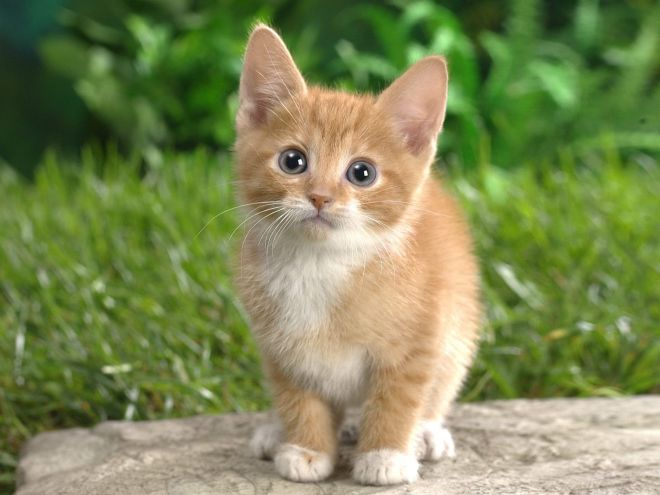
\includegraphics{Chapter1/figs/cat.jpg}
    \caption{Given an image, image classification algorithms try to output a label of the main object in that image. For instance, the label associated with this image is `cat'.}
    \label{fig:chap_1_cat}
    \vspace{-1em}
\end{wrapfigure}

To train such models, the currently predominant approach is \textit{supervised learning}: the model is provided with a dataset of labelled input-output pairs, and is then trained to minimise some error criterion on this dataset. This general paradigm of learning is very flexible, and can be applied to solve many tasks, with a wide variety of models. Indeed, many of the recent flourishings of applied machine learning lean on flexible model classes combined with large amounts of training data \citep{Krizhevsky:12,Wu:16}.

A famous dictum in the early days of statistical learning was `there's no data like more data'\footnote{Bob Mercer, 1985 \citep{Jelinek:05}}, and this trend has continued to the present day. ImageNet \citep{Deng:09}, one of the largest publicly available hand-annotated datasets, comprises \textit{14 million} annotated images collected over 8 years. Further, collecting annotations costs money, and the more specialised the annotation the more expensive it is. For example, SNLI, a large-scale natural language inference understanding dataset, cost around \$55,000 (S Bowman, personal communication) to annotate 500,000 examples; however, the annotation task was relatively straightforward and did not require experts to gather. On the other end of the spectrum, the Penn Treebank \citep{Marcus:93} used 15 graduate linguistics students to annotate 7 million words, and cost roughly \$10 million. A recent annotation effort for French syntax gives a rough figure of \euro{13} per sentence \citep{Martinez-Alonso:16}. Thus, annotating more and more data quickly becomes a time- and money-consuming enterprise, even though raw data is becoming more and more plentiful.

On the other hand, even unlabelled raw data contains much information about the state of the world, and it is conceivable that being able to learn from unlabelled data could benefit machine learning models. Indeed, there is evidence that free-form, undirected observation and interaction with the world (a.k.a. `play') is crucial for child development (\citet{Frost:98} and references therein). Therefore, approaches that can make use of unlabelled data to learn the structure of the world around us hold great potential in unlocking the power of raw data. This subfield of machine learning is called \textit{unsupervised learning}.

One potential approach in this vein is to instead learn to \textit{create} new data which resembles existing data. The core idea is that, just as a successful art forger needs to understand intricately the style of the artist they seek to emulate, so a successful `machine forger' needs to understand the underlying process which gives rise to the observed data. If the observed data comes from natural observations, then this necessarily involves some understanding of the hidden structure of nature.

For example, consider generating images of faces. To be successful at this, a model has to discover that there are independent factors of variation in human faces, such as eye colour and hair colour. In addition, it has to learn the possible eye and hair colours, and what correlations exist between them (such as dark hair predisposing towards darker eyes). Therefore, to do this successfully, the model has to discover the independent features of variation of the data, and how they co-vary; in short, the model has to `carve nature at its joints' \citep{Plato:52}.

In machine learning, models that can generate realistic data points are called \textit{generative models}. They have found wide use in machine learning, both in supervised tasks such as sentiment analysis \citep{Pang:02} and spam email filtering \citep{Pantel:98,Sahami:98}, and on unsupervised structure discovery tasks in fields such as text analysis \citep{Blei:03} and population genetics \citep{Pritchard:00}. Further, due to their ability to generate new data examples, generative models have also been used to explore computational creativity, in domains such as poetry generation \citep{Zhang:14,Ghazvininejad:16,Hopkins:17} and image style transfer \citep{Zhu:17}.

One particular class of generative models are latent variable models. Here, the observed data is assumed to be dependent on unobserved variables. This gives a probabilistic grounding to unsupervised learning techniques such as dimensionality reduction \citep{Tipping:99} and clustering \citep{Gorur:10}. In NLP, classic examples of latent variable models include probabilistic latent semantic analysis (PLSA) \citep{Hofmann:99} and latent Dirichlet analysis (LDA) \citep{Blei:03}. In addition, by encoding assumptions about the generative process in the structure of the latent variables, we can perform structure discovery with latent variable generative models, such as unsupervised dependency parsing \citep{Klein:04,Blunsom:10}. Finally, as latent variable generative models are inherently probabilistic, they gracefully handle output uncertainty well \citep{Kohl:18}.

The core problem of interest with latent variable models is inference on the latent variables given observed data. This is necessary both during learning (for algorithms such as EM \citep{Dempster:77}), and use (i.e. if we want to use the latent variables as data representations). However, calculating the posterior of the latent variables requires calculating the data likelihood. This requires integrating out the latent variables, which is in general infeasible. While closed form expressions for the posterior exist for certain model classes, this imposes harsh constraints on the form of the model, and rules out using interesting likelihood models, and in particular sequence models like recurrent neural networks (see next paragraph). Another option is approximating the integral using a sampling-based algorithm like Markov chain Monte Carlo ; however, this can have high variance, and requires multiple evaluations of the likelihood, which can be expensive. Alternatively, one can try to approximate the posterior with a simpler class of distributions, and try to select the distribution from this class that most closely matches the true posterior -- this approach is known as \textit{variational inference}. However, this approach is inherently suboptimal due to the approximation involved, and an inexpressive class of distributions can result in poor model fit. Further, selecting the optimal approximate posterior requires optimisation, which can be slow for large data sets.

All these reasons have meant that latent variable models, especially in NLP, have used simple likelihood models to keep inference and optimization tractable. However, over recent years, powerful general-purpose models have revolutionised the field of machine learning, and one particular class of models that have (re)gained traction in recent years are neural networks. These biologically inspired models have shown an incredible ability to scale with data \citep{Koehn:17}, in part due to their ability to universally approximate functions \citep{Cybenko:89}. One particularly appealing feature of neural networks is that they allow the parameterisation of complicated distributions, such as over images or sequences, without making the independence assumptions necessary in pre-existing literature.

An illustrative example of this is in the field of \textit{language modelling}, which assigns probabilities to sequences of words. The dominant approach towards language modelling is to use the chain rule of probability to rewrite the probability of a sequence as a product of individual conditional word probabilities, where the conditioning context is the previous words seen. This reduces the problem of learning a sequence predictor into learning a next word predictor.

The prehistory of language modelling was dominated by \textit{n-gram language models} \citep{Jelinek:76,Baker:90}. These use only the most recent $n$ words to guess the next word, and discard any context from further back than this. However, these models are fundamentally limited: human language contains arbitrary length dependencies in constructions like center embedding, and no $n$-gram model can fully capture these interactions. Indeed Noam Chomsky in a series of papers (starting with \citet{Chomsky:56}) argued against n-gram language models as a model for human cognitive processing of language. Neural networks, and in particular recurrent neural networks \citep{Elman:90,Hochreiter:97}, on the other hand, can encode arbitrary length contexts without making any independence assumptions \citep{Mikolov:10,Sundermeyer:12}. Due to this, they currently set the state of the art for language models when evaluated intrinsically using perplexity \citep{Melis:18}, although there is evidence to show that on huge datasets n-gram language models can still achieve competitive performance \citep{Chelba:17}.

% One particularly exciting application of neural networks is as the likelihood function of a generative model. This combination is broadly known as a \textit{deep generative model}. Early work in this area include Boltzmann machines \citep{Ackley:85}, and Helmholtz machines \citep{Dayan:95}. However, these models either require sampling to train, which can be slow, or do not optimise a valid bound on the data (log-)likelihood, which can lead to inconsistent parameter estimation.

Given these spectacular successes, a natural line of enquiry is whether we can combine neural networks and latent variable generative models. As with all neural network research, there is much early work on this area, including (restricted) Boltzmann machines \citep{Hinton:83,Ackley:85,Smolensky:86} and Helmholtz machines \citep{Dayan:95}. However, these models either require sampling to train \citep{Hinton:02,Tieleman:08}, or do not optimise a valid bound on the data log-likelihood \citep{Hinton:95}. Further, the model architectures considered only account for fixed-size outputs, and so previous applications of deep generative models to text still made strong word independence assumptions \citep{Hinton:09}.

Work in this area was revitalised by a central idea published contemporaneously by 3 different groups \citep{Kingma:14,Rezende:14,Titsias:14}. One problem with classic variational inference is that typically the parameters of the approximation to the true posterior were optimised independently for each data point. This results in an inner optimization loop inside the main optimization loop, which can be prohibitively slow for large data sets. However, one can view the optimal variational parameters as a function of the input data, and then try to approximate this function with a neural network. Further, we can train this neural network jointly with the generative model to optimize a valid bound on the data log-likelihood, using low-variance single sample gradient estimates of this bound with the \textit{reparametrization trick}. This combination of model, inference and learning is collectively known as a \textit{variational auto-encoder}, or VAE for short, due to similarities with classical autoencoders.

%This idea showed the way to train generative models of text without making restrictive independence assumptions. In particular, we can now train latent variable generative models with powerful sequence-level RNN likelihood functions, an approach first pioneered in \citet{Bowman:16}. These papers serve as the launching point of my thesis, where I explore applications of latent variable models in various NLP tasks.

The power of the variational autoencoder is that it provides a very general recipe to perform inference and learning in a wide range of generative model architectures. Building on this, \citet{Bowman:16} showed how to train latent variable generative models of text with autoregressive likelihoods, and demonstrated that the latent variables captured global information about the sentences. My thesis continues this line of work, and explores both modelling advances and applications of deep generative models of text.

\section{Thesis contributions}

This thesis contains three main contributions:

\begin{itemize}
    \item In Chapter \ref{chap:chatbot}, I present a latent variable model for generating responses in open-domain conversation. Here, the latent variables are continuous, with a Gaussian prior, and summarise the external unobserved factors that account for variation in reply to a given prompt. I give a brief overview of the history of conversational AI, present my contribution, and motivate why a latent variable model is an intuitive idea for open-domain conversation. I evaluate the diversity of the outputs the model produces compared to baseline approaches towards open-domain dialogue, and present some human evaluation to show that humans prefer the output generated by the latent variable model compared to a baseline.
    
    \item In Chapter \ref{chap:sentencelda} I present an extension to LDA which instead draws entire sentences from the latent topics. Here, the latent variables are discrete, and represent a semantic topic for the sentence. I outline the motivation behind doing so, and also discuss the engineering challenges behind optimising such a model, and how I overcame them. I demonstrate that the resulting model is a very powerful model of documents, with better perplexity scores than a wide range of existing latent-variable baselines. I also perform a qualitative analysis of the topics the model learns, and show that the topics the model learns are semantically coherent as judged by human annotators.
    
    \item In Chapter \ref{chap:amrgeneration}, I present a model for generating a surface form from a semantic representation by generating first a syntactic representation. Here, the latent variable is the syntax, which is a structured discrete latent variable. I show that factorising the model in this way leads to state-of-the-art results in AMR generation as measured by automated metrics. Further, we show that as our model has knowledge of syntax, we can generate syntactically varied realisations of the same underlying semantic form, and that human annotators prefer this variation over variation from a baseline model.
\end{itemize}

\section{Additional work not included in this thesis}

During my PhD, I have had the fortune to work on many topics, some of which did not fit into this thesis. In the interests of completeness, I shall talk briefly about those papers in this section, and try to sketch how they relate to the main theme of my thesis.

\subsection{A joint model for word embedding and word morphology}

\textit{This material first appeared in \citet{Cao:16}}

In this paper, I tackle the problem of word segmentation and word subunit discovery using distributional information. To do this, I propose a model that, given a proposed binary segmentation point in a word, composes the characters to the left and right of the point to obtain a representation of the segmented word. The representations of all possible binary segmentations are then combined with a weighted sum to obtain a representation for the word. The model is trained using the skip-gram with negative sampling objective from \citet{Mikolov:13}: I use  the composed word representations to predict context words. The intuition behind the model is that word segmentations which uncover morphemes give rise to representations which are helpful to predict neighbouring words and are thus upweighted, while random segmentations do not help predict context words and are downweighted. This model can be viewed as performing approximate inference in a latent variable model of context word prediction where the latent variables are proposed word segmentations.

I evaluated the model proposed segmentations against baseline word segmenters, and show that it achieves comparable segmentation accuracies to existing unsupervised morphological analyzers. I further evaluated the quality of the compositional word representations the model learns, and show that they outperform a baseline compositional word representation model on rare morphologically complex words, and also at the task of syntactic analogy solving. Finally, I qualitatively examine word nearest neighbours in embedding space, and show that the model learns both orthographic and semantic similarity.

\subsection{Emergent communication through negotiation}

\textit{This material first appeared in \citet{Cao:18}}

In this paper, I examine the possibility of two agents establishing a communication protocol to enable the division of a shared pool of items, with each agent having a differing value for each item. This is done entirely ground up: the only supervision signal the agents receive is the task reward at the end; that is, the value of the items each agent receives. We examine various forms of communication protocol, and various agent payoffs, and show that if the agents are self-interested (that is, receive reward only according to the items they themselves obtain) and communicate using 'cheap talk' (ungrounded symbols without \textit{a priori} semantics), they cannot learn to solve this task.
%!TEX root = ../thesis.tex
%*******************************************************************************
%****************************** Second Chapter *********************************
%*******************************************************************************

\chapter{Background}

\ifpdf
    \graphicspath{{Chapter2/Figs/Raster/}{Chapter2/Figs/PDF/}{Chapter2/Figs/}}
\else
    \graphicspath{{Chapter2/Figs/Vector/}{Chapter2/Figs/}}
\fi

\section{Neural networks}

\textit{The history of neural networks is convoluted and winding, and it is difficult to give a concise overview of their history. What follows is a synchronic description of how they are used -- a brief historical overview follows in the next section.}

\subsection{A brief practitioner's guide to neural networks for NLP}

Neural networks are nonlinear function approximators of a certain shape: they perform an affine transformation of the input, followed by a non-linear function, to obtain an output. In this view, logistic regression corresponds to the simplest class of neural networks, with the choice of non-linearity being the logistic function. To exclude cases like this, typically one adds the condition that one composes multiple functions of the above form to obtain the input-output function. This creates \textit{hidden layers}: the intermediate states in the chain of non-linear affine transformations.

The simplest example of a neural network is when the affine transformation is a simple matrix multiplication followed by a translation. This is referred to as a \textit{feedforward layer}. An alternative is to convolve the input with a small kernel: a matrix much smaller than the input size. This gives rise to a \textit{convolutional layer}, the building block of a \textit{convolutional neural network}. These have been tremendously successful in image processing and speech recognition recently @@@cite, and have also been applied for 

One notable fact about neural networks is that, with one hidden layer of infinite width, they are able to universally approximate any function \citep{Cybenko:89,Hornik:91} under mild assumptions on the non-linearity. This provides one justification for their use: given enough hidden units, they can learn any input-output mapping in a supervised task.

One recent 

A neural network consists of two parts: an architecture, and a learning algorithm. Typically, the structure of a neural network can be represented by a directed acyclic graph. Nodes without incoming edges are input nodes, which is how information is fed into the neural network. Nodes without outgoing edges are output nodes, which represent the network's computation on the input. Each node, or \textit{neuron}, takes all input values from incoming connections, does some computation on these input values, and stores the result as its output value. Commonly, one multiplies each incoming value by a \textit{weight}, and then sums them up to form an intermediate value. Classically (e.g. the perception), this intermediate result would be compared to a threshold: if the intermediate was greater than the threshold, the neuron would output 1, otherwise the neuron would output 0. If we denote by $\mathbf{x}$ the vector of input values for a neuron, this corresponds to the neuron computing the following function:
\begin{equation}
    f(\mathbf{x}) = H(\mathbf{w} \cdot \mathbf{x} + b)
\end{equation}
where $H$ denotes the Heaviside step function, $\mathbf{w}$ the vector of weights for the incoming connections, and $b$ the (negative) threshold (also called the \textit{bias}). For optimisation reasons (see later), it is often preferable to have a differentiable non-linearity. Thus, sigmoid, tanh or ReLU non-linearities are often used in contemporary neural networks.

\subsection{Common neural network architectures in NLP}

Different graph structures give rise to different neural network architectures. At present, it is most common to organise the nodes into successive \textit{layers} $l_1, \dots, l_n$ such that neurons in each layer only have incoming connections from nodes in the previous layer and outgoing connections to nodes in the subsequent layer. This also makes it easier to implement neural networks, as the computations for each layer can be calculated as affine transformations, which take advantage of optimized matrix-vector and matrix-matrix multiplication routines.

The most basic instantiation of the above architectures has (possibly many) layers of nodes, with each node in each layer connected to all nodes in the preceding and subsequent layers. This is known as a \textit{fully-connected network}. Another variant which reignited interest in neural network models for vision is called a \textit{convolutional neural network}. Here, a small window of neurons (called a \textit{filter}), with the same incoming weights and biases, are scanned over an input incrementally, based on the intuition that visual features tend to be local and translation-invariant within an image. These networks appear to learn low-level visual features in early layers, such as edges and basic shapes, while higher layers seem to capture more global semantic information. @@@cnns for text: n-gram features (whether over words or characters).

Neural networks can also contain self connections, where the state of a layer is computed based on its state in the previous timestep. This introduces recurrence into the network, and networks with these connections are called \textit{recurrent neural networks} (RNNs). These models are particularly useful for models with sequential structure, such as text, as the hidden state at a particular timestep depends on all previous timesteps, and in effect acts as a kind of memory. The most basic instantiation of RNNs are Elman recurrent networks. Here, the hidden state at time $t$ depends on both the hidden state at the previous timestep and the current input:
\begin{equation}
    h_t = f(W h_{h-1} + U x_t + b)
    \label{eqn:rnn}
\end{equation}
where $f$ is a non-linearity. This update rule rewrites the memory of the network at each timestep, and hence makes long-term temporal credit assignment difficult (cf. the vanishing/exploding gradients problem).

Hochreiter and Schmidthuber @@@cite proposed a solution by including another memory state in the recurrence: the \textit{cell state}. This is only written to additively, and this helps prevent the vanishing/exploding gradient problem. Concretely, this changes the RNN update rule (Equation \ref{eqn:rnn}) to the following:
\begin{align}
    f_t &= \sigma(W_f h_{t-1} + U_f x_t + b_f) \\
    i_t &= \sigma(W_t h_{t-1} + U_t x_t + b_i) \\
    o_t &= \sigma(W_o h_{t-1} + U_o x_t + b_o) \\
    c_t &= f_t c_{t-1} + i_t \tanh(W_c h_{t-1} + U_c x_t + b_c) \\
    h_t &= o_t \tanh(c_t)
\end{align}
where $\sigma$ is the sigmoid function, and all vector-vector products are to be intepreted pointwise. The intuition is that $c_t$ represents the long-term memory of the network, and reading and writing to this is performed additively. $i_t$ and $f_t$ are the input and forget gates respectively, which guard how much of the previous timestep's cell state is kept and overwritten respectively. $o_t$ is the output gate, which controls how much of the cell state is exposed as the new hidden state. Note that the previous timestep hidden state is only indirectly used to calculate the new hidden state.

Due to the sequential nature of RNN processing, the hidden state at time $t$ can only consider inputs at time less than $t$. However, for some tasks, knowledge of future inputs can be useful, such as disambiguating noun/verb word senses for POS tagging. A simple way to incorporate future context is to process the input in reverse order with another RNN to obtain a sequence of hidden states $h_t^{rev}$, where each $h_t^{rev}$ captures the forward context of the word to the end of the sentence. Then, the forward and reverse hidden states are concatenated to obtain the final hidden state $h_t$ at time $t$. This is known as a bidirectional RNN, and the reverse RNN effectively acts as a powerful lookahead feature extractor @@@cite.

One of the major uses of neural networks in NLP is representation learning, especially for sentences. As neural networks compute using vectors of real numbers, the final hidden state of the neural network after processing an entire sentence can be used as a feature vector to a linear model. This can be either the final hidden state of an RNN or LSTM scanning over the sentence, or the final hidden layer of a stack of convolutions. The neural network acts as an encoder, compressing the variable length input into a fixed-width representation. 

A particularly important application of sentence representation learning is in the sequence-to-sequence framework. In many conditional language generation tasks, such as machine translation, we often need to generate language from structured input data. The sequence-to-sequence approach encodes the input data using a neural network to a vector representation, which is then fed into a neural language model decoder which generates the output text one word at a time. This approach demonstrates the modularity and flexibility of neural networks, as one can use a wide range of network architectures in both the encoder and decoder.

One issue with the above approach is that the same dimension vector is used to represent every sentence, no matter what length the sentence is. For long sentences, therefore, there is information loss in the compression process, and empirically the performance of a simple sequence-to-sequence model on translating long sentences is poor. To bypass this bottleneck, @@@Bahdanau propose the \textit{attention} mechanism, where the encoding of the input is dynamically computed during decoding. In detail, rather than encoding the input as a single vector, an attentional model encodes the input as a sequence of vectors $c_1, \dots, c_n$, called annotations. Then, at timestep $t$ during decoding, the decoder uses its current hidden state, $h_{t-1}$, to query the annotations, and then uses the (normalised) query scores as weights to calculate the context vector for the current timestep. This context vector is then fed into the LSTM recurrence:
\begin{align}
    a_i &= \text{sim}(h_{t-1}, c_i) \\
    w_i &= \frac{a_i}{\sum a_i} \\
    s_t &= \sum w_i c_i
    h_t = LSTM(h_{t-1}, x_t, s_t)
\end{align}

Many choices of similarity function have been proposed. The original paper used a multi-layer perceptron to calculate the similarity score, while @@@luong showed that a bilinear scoring function performed better in machine translation empirically.

\subsection{Feature representation in neural networks}

Neural networks manipulate vectors of real numbers. Therefore, when processing language with neural networks, one fundamental consideration is how to represent the symbolic language input in a format amenable to neural computation. There are issues to do with the granularity of the input (what scale do we discretise the language) and coding (how do we represent the discretised units of language numerically).

For many languages, words appear to be the basic unit of language, and indeed many languages are written word-segmented, such as English. This suggests processing language on the word-level, and using words as input features. This is the standard approach for contemporary NLP. However, for many languages, such as Chinese, words are not segmented when written. This means that an additional tokenisation step has to be run, which may introduce errors into the pipeline. Further, due to the long tail of language, particularly for languages with rich morphology, storing a separate feature for each word results in a prohibitive number of features, and many words will not be seen more than once in the training data\footnote{In the standard training split of the Wall Street Journal corpus, xx\% of words are hapax legomena}. To deal with this, typically we limit the word features to the most frequent $k$ words in the training corpus, or take only words which appear more than $n$ times. Even if we use all words seen in the training data as features, we can expect to find many words in test data which have not been seen in the training data, and representing these unseen words poses a challenge.

One approach is to use a special cover token (typically denoted UNK, for UNKnown word) to represent all unseen words, and train the model using this feature by replacing certain words in the training data with this token. However, this approach completely disregards any information contained in the unseen token. Another approach is to incorporate additional features into our input apart from just word identity. For example, many parsing models @@@ make use of additional capitalisation and part-of-speech features, which are represented by a binary feature and an index into a closed vocabulary respectively. 

To help deal with the word sparsity issue, sub-word level features can also be used. Morphemes, being the minimal unit of meaning, make appealing features, as they contain both semantic information in the lemma and any derivational affixes, as well as syntactic information in inflectional affixes. This helps smooth over the rare-word issue, as many words in the long tail tend to be morphologically related to high frequency words. However, breaking down words into morphemes is a tricky process: hand-written morphological analysers are brittle and require lots of engineering effort, while (minimally) supervised approaches are still fairly error-prone. The most extreme approach is to use the raw characters of the word as input features. This bypasses the issue of having to provide a morphological analysis, but requires a powerful model to capture the (largely arbitrary) form-meaning mapping. Some models elect to use a combination of features, and indeed including character level features and a powerful character composition model (such as an RNN or a CNN) can often increase performance across a wide range of NLP tasks @@@cite.

Whichever features we choose, we must turn them into a numerical representation to feed into a neural network. The typical way of doing this is using \textit{one-hot coding}. This represents features as a sparse vector of dimension the total number of features, with a 1 at the dimension corresponding to the index of the feature and 0's elsewhere. If there are multiple disjoint sets of features, such as word and POS features, they are typically one-hot coded separately, and then the resulting one-hot vectors are concatenated before being fed into the model. This means that the first weight layer of the neural network is effectively a lookup table which associates each feature with a vector called an \textit{embedding}. 

One special class of embeddings are the representations a neural network learns for word features. These are called \textit{word embeddings}, and they can be initialised randomly and trained with the rest of the network. However, many datasets are small, and so words which appear few times in the training corpus may have their parameters badly estimated during the training procedure. An alternative is to pretrain word embeddings on an unsupervised task using copious amounts of unlabelled data and use these to initialise the model word embedding parameters. This simple technique can be viewed as a cheap way of doing semi-supervised learning, and has been shown to improve performance at a wide range of NLP tasks (@@@cite).

Word embedding pretraining typically involves some form of language modelling objective. The earliest approaches took the word embedding parameters from a neural language model; however, with a large vocabulary, language modelling can be computationally intensive. Consequently, a plethora of methods for efficient neural langauge model training have been published (@@@cite hierarchical softmax, importance sampling, NCE). @@@Mikolov introduced a new unsupervised paradigm: instead of predicting the next word given the context, decide whether two words appear in the same context or not. This avoids computing the softamx entirely, and resulted in orders of magnitude speedups for word embedding estimation.

An alternative approach is to derive word embeddings directly from word cooccurrence counts. Latent semantic analysis performs an SVD factorisation of a word-word cooccurrence matrix, and uses the resulting low-dimensional vectors as word representations. Another popular word embedding model, GLoVE @@@cite, also can be viewed as an enhanced matrix factorisation model which factorises the log-probability of word coccurence rather than the raw cooccurence count. 

One interesting phenomenon of all of these models is that geometric similarity of words in the embedding space seems to reflect the underlying conceptual similarity of those words. This is perhaps explained by the \textit{distributional hypothesis}, which states that words which occur in similar contexts tend to have similar meanings. Indeed, the embedding space can be viewed as a form of \textit{conceptual space} @@do more here.

\subsection{Training neural networks}

The second component of a neural network is the learning algorithm. This specifies how the neural network should adapt to the training data in order to minimise some error criterion. While many different learning rules have been proposed in the literature, the \textit{de facto} standard currently is gradient descent on the parameters (i.e. the weights) of the neural network to minimise some loss function. Common loss functions include the cross-entropy between the model prediction and the true label, or margin-based losses between the model prediction and the ground truth.

A naive approach towards calculating the gradients of the loss function with respect to the model parameters is quadratic in the number of layers, as we would have to effectively traverse the computational graph for each layer. However, if we memoise the intermediate steps, we can calculate all of the derivatives in one backwards pass through the network. This is the basic idea behind the backpropagation algorithm, which in practice is how derivatives are computed for neural networks. 

Once gradients are calculated, the parameters have to be updated. One common way of doing this is to use (minibatched) stochastic gradient descent (SGD): for a parameter $\theta$, with gradient $\nabla\theta$, the update is
\begin{equation}
    \theta \leftarrow \theta + \alpha \nabla \theta
    \label{eqn:sgd}
\end{equation}
where $\alpha$ is the \textit{step size}, which is a hyperparameter of the SGD algorithm. Minibatch here refers to the fact that typically, purely online SGD (calculating gradients based on one training set example at a time) suffers too much from variance in the gradient, while fully batched SGD is too memory-intensive. Thus, the gradient estimate $\nabla\theta$ in Equation \ref{eqn:sgd} is calculated using a small batch of data points\footnote{in the order of 32-100 examples} sampled from the training data.

Pure SGD can have problems converging in certain pathological conditions, such as very flat minima. A commonly used variant introduces a momentum term to accelerate convergence, which simulates the behaviour of a heavy ball under gravity. This changes the update rule to:
\begin{align}
    z &\leftarrow \beta z + \nabla \theta \\
    \theta &\leftarrow \theta + \alpha z
\end{align}
where now we introduce another hyperparameter $\beta$, which controls how strongly we remember previous gradients. In practice, momentum appears to speed up the convergence of gradient descent, and makes SGD more resilient to choices of the step size hyperparamater.

Typical convergence proofs of SGD require the step size hyperparameter to go to zero over the course of optimisation. There are many ways of scheduling the learning rate, such as epoch-based, or by monitoring performance on a held-out development set; these all add to the number of hyperparameters which need to be tuned. Adaptive learning rate algorithms (@@@cite adagrad, adadelta, adam) attempt to automatically schedule the learning rate using convergence information. They also claim to be more resilient to hyperparameter choices. Although well-tuned SGD with momentum typically performs better than using an adaptive optimizer with off-the-shelf hyperparameter settings, the latter perform well enough to justify the convenience.

As neural networks are low-bias function approximators, they overfit very easily. Regularisation is therefore crucial to good model performance. There are many common regularisation techniques for neural networks: one common one is $\ell_2$-regularisation, which penalises weights with high $\ell_2$ norm. The most widely used technique is dropout @@@cite. Here, a proportion of the output values in each layer are randomly zeroed out. This was originally presented to be an empirically effective technique, but the theoretical motivation was lacking. @@@gal derived connections between dropout and variational inference, and showed how dropout can also give uncertainty estimates out-of-the-box, and also how to apply dropout to self-connections in neural networks. @@@gabor showed that, when properly regularised, LSTM models outperform more complicated architectures at language modelling, which highlights the power of dropout.

\section{Generative models}

In machine learning, generative modelling is the name given to a class of approaches which try to learn the distribution of the data. For a classification task, this involves learning the joint distribution of inputs $X$ and the labels $Y$; stretching the definition, generative modelling can also mean capturing the distribution of given data $X$ in unsupervised learning with a view towards drawing samples from the learnt model which resemble actual data points. One of the most common ways of specifying a generative model is as a graphical model, where nodes represent random variables and edges represent dependence relations.

Another application of generative models in NLP is parsing. PCFG-based parsers

@@@generative parsing models?

\section{Deep generative models}

Deep generative models are a class of approaches towards generative modelling which make heavy use of neural networks to parametrise certain components of the model. 

The earliest generative models which use neural networks were Hopfield networks, and their stochastic counterparts Boltzmann machines. These define the energy of a configuration, which corresponds to an unnormalised log-probability. Training a Boltzmann machine corresponds to increasing the probability of the training data. @@@computing normalising constant is hard, have to use gibbs sampling or contrastive divergence

Restricted Boltzmann machines (RMBs) aim to alleviate the difficulty of training general Boltzmann machines by making the node structure bipartite. One set of nodes corresponds to the input data, and the other are the `hidden' or latent layer. This simplifies sampling from the model, as now we can use blocked Gibbs sampling to sample either the input nodes or the latent nodes in one go. As an added bonus, inferring the most likely latent variable configuration for a given input gives us a low-dimensional `representation' of the input.

However, inference in RBMs is still difficult, as calculating the normalising constant requires summing over exponentially many configurations in the number of total nodes. While sampling-based Monte Carlo approaches can be used, it is often difficult to tell whether the samples are of good quality. An alternative approach is to use variational approaches to perform approximate inference. @@@

@@@variational autoencoder, generative adversarial network
%!TEX root = ../thesis.tex
%*******************************************************************************
%****************************** Third Chapter **********************************
%*******************************************************************************
\chapter{Latent Variable Dialogue Models and their Diversity}
\label{chap:chatbot}

% **************************** Define Graphics Path **************************
\ifpdf
    \graphicspath{{Chapter3/Figs/Raster/}{Chapter3/Figs/PDF/}{Chapter3/Figs/}}
\else
    \graphicspath{{Chapter3/Figs/Vector/}{Chapter3/Figs/}}
\fi

\section{Introduction}

The ability to engage in human-level conversation has long been considered a hallmark of intelligence -- indeed, the Turing test \citet{Turing:50} proposes the ability to imitate a human in conversation as an operational definition of artificial general intelligence. ELIZA \citep{Weizenbaum:66} was one of the first attempts at building a conversational AI agent that could pass the Turing test. @@@add description of eliza here.

One shortcoming of ELIZA was that its most convincing incarnations were based on narrow domains, specifically psychotherapy. The nature of Rogerian therapist interactions, with the therapist essentially acting as a reflection of the patient, lends itself to shallow pattern-matching based approaches towards understanding. This approach towards `cheating' the Turing test continued, with rule-based approaches successfully convincing a human interlocutor that the AI was a schizophrenic and a 13-year old non-native English speaker @@@citations.

Template-based chatbots proliferated after ELIZA, each usually having some idiosyncrasy to disguise the scripted nature of the conversation @@@add citations. However,  As AI and NLP in general moved away from rule-based systems towards statistical learning-based approaches, so did conversation agent research. \citet{Ritter:11} was one of the early pioneers of this line of research, using statistical machine translation techniques to transform a given conversational prompt into a response.

As neural approaches towards machine translation supplanted traditional phrase-based approaches, research into neural approaches towards open-domain conversational dialogue picked up steam \citep{Shang:15,Vinyals:15,Jiwei:16b,Jiwei:16,Serban:16}. Most previously published models train to minimise the negative log-likelihood of the training data, and then at generation time either perform beam search to find the output $Y$ which maximises $P(Y|\mathrm{input})$ \citep{Shang:15,Vinyals:15,Serban:16} (ML decoding), or sample from the resulting distribution \citep{Serban:16}. 

A notorious issue with ML decoding is that this tends to generate short, boring responses to a wide range of inputs, such as \textit{``I don't know"}. These responses are common in the training data, and can be replies to a wide range of inputs \citep{Jiwei:16,Serban:16}. In addition, shorter responses typically have higher likelihoods, and so wide beam sizes often result in very short responses \citep{Tu:2017,Belz:2007}. To resolve this problem, \citet{Jiwei:16} propose instead using maximum mutual information with a length boost as a decoding objective, and report more interesting generated responses.

Further, natural dialogue is not deterministic; for example, the replies to \textit{``What's your name and where do you come from?''} will vary from person to person. \citet{Jiwei:16b} have proposed learning representations of personas to account for inter-person variation, but there can be variation even among a single person's responses to certain questions.

Recently, \citet{Serban:17} have introduced latent variables to the dialogue modelling framework, to model the underlying distribution over possible responses directly. These models have the benefit that, at generation time, we can sample a response from the distribution by first sampling an assignment of the latent variables, and then decoding deterministically. In this way, we introduce stochasticity without resorting to sampling from the decoder, which can lead to incoherent output -- see Table \ref{tab:outputs} for examples.

In this paper, we present a latent variable model for one-shot dialogue response, and investigate what kinds of diversity the latent variables capture. Our experiments show that our model has higher lexical as well as sentential diversity than baseline models. We also show that our model generates more acceptable diverse output than sampling from a deterministic decoder. We end by noting that all three methods proposed above to combat the `maximum likelihood response' are ways of decreasing the probability of the generated output, and report some preliminary results for how response probability interacts with grammaticality and interestingness.

\section{A Latent Variable Dialogue Model}

\begin{table*}[t]
\centering{
\resizebox{\textwidth}{!}{
\begin{tabular}{p{0.3\textwidth} | l l}
\toprule
    Prompt & \textsc{Dial-LV} & Sampling ($\tau=1.0$) \\
\midrule
    \multirow{3}{*}{\pbox{0.3\textwidth}{the infection's spreading.}} 
        & he's dead. & he was lee . \\
        & nothing but no more. & leave it a way. \\
        & i know what you're doing & there's something going on in the phone rickshaw and put the afloat continuously... \\
\midrule
    \multirow{3}{*}{\pbox{0.3\textwidth}{we only have fourteen hours to save the earth!}}
        & i've got no choice . & can i win? \\
        & and then there's something that's what it's like. & go peacekeeper go. \\
        & well, we need the help of what's happening. & go to say hello again in this conversation. \\
\midrule
    \multirow{3}{*}{\pbox{0.3\textwidth}{why don't i do some research and send you an email?}}
        & well, we're gonna have to make it. & no disrespect team. \\
        & because i know how much it is. & excuse me. \\
        & because it 's not right. & because i'm hotel. \\
\bottomrule
\end{tabular}
}
}
\caption{3 random outputs for 3 random prompts from the dataset from our proposed model (\textsc{Dial-LV}) and naively sampling from the decoder of a deterministic encoder-decoder.}
\label{tab:outputs}
\end{table*}

\subsection{Model Description}
Our task is to model the true probability of a response $Y$ given an input $X$. We denote our model distribution by $P(Y | X)$. We introduce a latent variable $z$ with a standard Gaussian prior  -- i.e. $P(z) = \mathcal{N}(0, I_n)$ -- and factor $P(Y | X)$ as:
\begin{equation}
    P(Y | X) = \int_{z} P(Y | z, X) P (z) dz
\label{eqn:chain_rule}
\end{equation}

To motivate this model, we point out that existing encoder-decoder models encode an input $X$ as a single fixed representation. Hence, all of the possible replies to $X$ must be stored within the decoder's probability distribution $P(Y|X)$, and during decoding it is hard to disentangle these possible replies.

However, our model contains a stochastic component $z$ in the decoder $P(Y | z, X)$, and so by sampling different $z$ and then performing ML decoding on $P(Y | z, X)$, we hope to tease apart the replies stored in the probability distribution $P(Y|X)$, without resorting to sampling from the decoder. This has the benefit that we use the decoder at generation time in a similar way to how we train it, making it more likely that the output of our model is grammatical and coherent. Further, as we do not marginalize out $z$ when decoding, we no longer perform exact maximum likelihood search for a reply $Y$, and so we hope to avoid the boring reply problem.

At training time, we follow the variational autoencoder framework \citep{Kingma:14,Kingma:14b,Sohn:15,Miao:16a} , and approximate the posterior $P(z | X, Y)$ with a proposal distribution $Q(z | X, Y)$, which in our case is a diagonal Gaussian whose parameters depend on $X$ and $Y$. We thus have the following evidence lower bound (ELBO) for the log-likelihood of the data:
\begin{multline}
    \log P(Y | X) \geq -\mathcal{KL} (Q(z | X, Y) || P(z)) \\ + \mathbb{E}_{z \sim Q} \log P(Y | z, X)
\end{multline}

Note that this loss decomposes into two parts: the KL divergence between the approximate posterior and the prior, and the cross-entropy loss between the model distribution and the data distribution. If the model can encode useful information into $z$, then the KL divergence term will be non-zero \citep{Bowman:16}. As our model decoder is given a deterministic representation of $X$ already, $z$ will then encode information about the variation in replies to $X$.

\subsection{Model Implementation}

\begin{figure}[t]
    \centering
    \includegraphics[width=\columnwidth]{model_implementation}
    \caption{A schematic of how our model is implemented. Please see the text for full details.}
    \label{fig:model_implementation}
\end{figure}

Given an input sentence $X$ and a response $Y$, we run two separate bidirectional RNNs over their word embeddings $\mathbf{x}_i$ and $\mathbf{y}_i$. We concatenate the final states of each and pass them through a single nonlinear layer to obtain our representations $h_{\mathbf{x}}$ and $h_{\mathbf{y}}$ of $X$ and $Y$. We use GRUs \citep{GRU} as our RNN cell as a compromise between expressive power and computational cost.

We calculate the mean and variance of $Q$ as:
\begin{equation}
\begin{split}
   \mu & = W_{\mu} [h_{\mathbf{x}} \ h_{\mathbf{y}}] + b_{\mu} \\
   \log(\Sigma) & = diag(W_{\Sigma} [h_{\mathbf{x}} \ h_{\mathbf{y}}] + b_{\Sigma})
\end{split}
\end{equation}
where $[a \ b]$ denotes the concatenation of $a$ and $b$, and $diag$ denotes inserting along the diagonal of a matrix.

We take a single sample $z$ from $Q$ using the reparametrization trick \citep{Kingma:14}, concatenate $h_{\mathbf{x}}$ and $z$, and initialize the hidden state of the decoder GRU with $[h_{\mathbf{x}} \ z]$. We then train the decoder GRU to minimize the negative log-likelihood of the response $Y$.

While training this model, we noted the same difficulties as \citet{Bowman:16} -- as RNNs are powerful density estimators, the model will prefer to ignore the latent variables and instead optimize the data reconstruction term of the ELBO, while forcing the KL term to 0. We overcome this using similar techniques by gradually annealing the KL term weight over the course of model training and using word dropout in the decoder with a drop rate of $0.5$.

\section{Experiments}

We compare our model, \textsc{Dial-LV}, to three baselines. The first is an encoder-decoder dialogue model with ML decoding (\textsc{Dial-MLE}). The second baseline model implements the anti-LM decoder of \citet{Jiwei:16} (\textsc{Dial-MMI}) on top of the encoder-decoder, with no length normalization. For these models, we use beam search with a width of 2 to find the sentence $Y$ which maximises the decoding objective (either ML or MMI).

The final baseline uses the encoder-decoder model, but instead samples from the decoder to find $Y$ (\textsc{Dial-Samp}). We found that naively sampling from the decoder resulted in meaningless jumbles of words. To solve this, we introduced a temperature parameter $\tau \in (0, 1]$, which scales the probability of each word of the decoder as $p_w \mapsto p_w^{1/\tau}$. This parameter serves to sharpen the word distribution of the decoder. We found $\tau = 0.35$ to be a reasonable balance between preserving stochasticity while also improving the coherence of the generated output.

We used the OpenSubtitles dataset of movie subtitles to train our models \citep{Tiedeman:12}. We took a random sample of 100K files from the full dataset to train our models on, and then pruned this of repeated files to leave roughly 95K files and capped sentence length to 50. The total size of the resulting corpus was around 731M tokens. Please see the supplementary material for model hyperparameters and training details.

As seeds for our replies, we used a list of 50 prompts: 150 lines from the OpenSubtitles dataset outside of our training set which we judged to make sense as independent sentences and 50 questions chosen from a list of suggested conversation starters\footnote{Obtained from http://conversationstartersworld.com/250-conversation-starters/}.

\subsection{Reply statistics}

\begin{table}[t]
\centering{
\resizebox{\columnwidth}{!}{
\begin{tabular}{c|cccc}
\toprule
     Model & Zipf parameter & NLL & Unique \% \\
\midrule
     \textsc{Dial-Lv} & 1.39 & 15.54 & 76 \\
     \textsc{Dial-MLE} & 1.43 & 12.15 & 35 \\
     \textsc{Dial-MMI} & 1.60 & 15.12 & 62 \\
     \textsc{Dial-Samp} & 1.53 & 16.66 & 78 \\
\bottomrule
\end{tabular}
}
}
\caption{Some statistics pertaining to the responses generated by the models.}
\label{tab:statistics}
\end{table}

Previous work (e.g. \citet{Jiwei:16}) used type-token ratio (TTR) to measure the diversity of the generated output. However, as language follows a Zipf distribution, TTR is affected by the length of the generated replies \citep{Mitchell:2015}. Hence, we use the estimated parameter of a Zipf distribution fitted to our replies as a proxy for the lexical diversity of generated output, with more diverse output having smaller scores. As ML decoding is known to give the same few replies repeatedly, we also report the percentage of unique replies, as a coarser measure of sentential diversity compared to lexical diversity. Further, we give the negative log-likelihood (NLL) as predicted by the deterministic encoder-decoder model, to see what regions of the probability space the replies occupy. We present these statistics in Table \ref{tab:statistics}. 

We note that \textsc{Dial-LV} generates more diverse replies than the other deterministic models, measured in terms of percentage of unique responses. Interestingly, the lexical diversity of \textsc{Dial-LV} is almost identical to \textsc{Dial-MLE}, suggesting that the latent variables help \textsc{Dial-LV} avoid the boring output problem and generate more diverse outputs. We note that \textsc{Dial-LV} even rivals \textsc{Dial-Samp} in terms of sentential diversity, and beats \textsc{Dial-Samp} in terms of lexical diversity. This could be because \textsc{Dial-Samp} chooses words greedily, and so is biased towards choosing high-probability words at each timestep. This suggests that maintaining a beam of hypotheses while sampling could help sampling-based methods escape the trap of having to make near-greedy local decisions.


\subsection{Human acceptability judgments}

\begin{table}[t]
\centering{
\resizebox{\columnwidth}{!}{
\begin{tabular}{c|ccccc}
\toprule
     Model & $\mu$ & $\sigma$ & NLL & Zipf & Unique \% \\
\midrule
     \textsc{Dial-LV} & 1.183 & 0.402 & 15.51 & 1.32 & 76.4 \\
     \textsc{Dial-Samp} & 1.196 & 0.577 & 16.91 & 1.56 & 73.6 \\
\bottomrule
\end{tabular}
}
}
\caption{Mean and std. dev. of average number of acceptable replies generated by each model.}
\label{tab:acceptability}
\end{table}

We also tested whether \textsc{Dial-LV} could generate a greater number of acceptable replies to a prompt than \textsc{Dial-Samp}. We randomly selected 50 prompts from our list of 200, and generated 5 replies at random to each one using both models. We then asked human annotators\footnote{We used 50 in total, 25 for each model} to judge how many replies were appropriate replies, taking into account grammaticality, coherence and relevance. The results are shown in Table \ref{tab:acceptability}.

Interestingly, even though \textsc{Dial-LV} has a lower NLL score, both models generate roughly the same number of acceptable replies. \textsc{Dial-LV} also has less variance in the number of acceptable replies, suggesting that the outputs it generates are more consistent than responses from \textsc{Dial-Samp}. Finally, we note that \textsc{Dial-LV} generates more diverse output than \textsc{Dial-Samp} in this scenario, even thought its replies are judged equally acceptable, suggesting that it is managing to produce a wide range of coherent, fluent and appropriate output.

\subsection{Sampling from the latent variable space}

\begin{table}[t]
\centering{
\resizebox{\columnwidth}{!}{
\begin{tabular}{c|ccc}
\toprule
     Shell radius & Zipf parameter & NLL & Unique \% \\
\midrule
     0 & 1.49 & 13.12 & 7 \\
     4 & 1.62 & 14.02 & 42.1 \\
     8 & 1.59 & 15.72 & 63.1 \\
     12 & 1.56 & 17.65 & 67.7 \\
     16 & 1.78 & 18.16 & 67.1 \\
\bottomrule
\end{tabular}
}
}
\caption{Statistics of responses generated from the \textsc{Dial-LV} model from different regions of the hidden state space.}
\label{tab:variety}
\end{table}

We next explored the effect of sampling from different regions of the latent space. For each prompt in the test set, we took 5 uniform samples from shells of radius 0 (which collapses to deterministic decoding), 4, 8, 12 and 16 in the latent space\footnote{For a $d$-dim standard Gaussian, $\mathbb{E}(\|X\|) \approx \sqrt{d}$, and $Var(\|X\|) \to 0$ as $d \to \infty$. Here $d=64$.} by sampling from $P(z) = \mathcal{N}(0, I)$ and then scaling the sample $z$ by the appropriate amount. We then generated a response to the prompt using each value of $z$, and measured some statistics of the replies. The results are shown in Table \ref{tab:variety}.

As expected, samples with small radius show less diversity in terms of unique outputs. Further, we see a consistent trend that samples with greater radius have a higher NLL score, showing the influence of the prior in Eqn. \ref{eqn:chain_rule}. However, at the highest radius, we observe the highest NLLs, but also the lowest lexical diversities, suggesting that it manages to combine the words it produces in many different ways.

\section{Discussion}
\label{sec:discussion}
Taken together, our experiments show that ML decoding does not seem to be the best objective for generating diverse dialogue, and so corroborates the inadequacy of perplexity as an evaluation metric for dialogue models \citep{Liu:2016}. Indeed, all three models which show a diversity gain over the vanilla encoder-decoder with MLE decoding try to instead sample responses from a lower-probability region of the response space. However, if the response probability is too low, it runs the risk of being nonsensical. Hence, there appears to be a `Goldilocks' region of the probability space, where the responses are interesting and coherent. Finding ways of concentrating model samples to this region is thus a potentially promising area of research for open-domain dialogue agents.

We also note that our proposed model can be combined with MMI decoding or temperature-based sampling to get the benefits of both worlds. While we did not do this in our experiments in order to isolate the impact of our model, doing so improves the diversity of our generated output even more.

\section{Conclusion}
In this paper, we present a latent variable model to generate responses to input utterances. We investigate the diversity of output generated from this model, and show that it improves both lexical and sentential diversity. It also generates more consistently acceptable output as judged by humans compared to sampling from a decoder.
\chapter{A sentence-level extension to LDA}
\label{chap:sentencelda}

\section{Introduction}

Generative models of text, such as latent Dirichlet allocation \citep{Blei:03}, seem to automatically capture the semantic content of collections of documents \citep{Griffiths:04}. These models typically assume documents are bags of words, with individual words only weakly correlating with one another, if at all. However, word meaning is dependent on context -- \textit{\textbf{support} vector machine} means something very different to \textit{generous \textbf{support}}. Therefore, modelling dependencies between words would allow these models to closer reflect the underlying text.

In this paper, we propose to use sentences, not words, as the basic exchangeable unit of topic models. We present two generative models of language which both generate whole sentences from the latent topics, replacing the topic-word categorical distribution with a more flexible topic-sentence distribution given by a recurrent neural network language model. We aim to capture intra-sentential dependencies such as syntax and compositional semantics using the RNN, and sentence-level semantics in the latent topics. Our models can be viewed as integrating language modelling into topic models.

One model, \textsc{sentVAE}, is a discrete hidden variable generative model of sentences. Here, for each sentence $s_i$ in a document $\mathcal{D}$, the model independently draws a topic $z$ from a uniform prior, and then draws a sentence from $z$. The other, \textsc{sentLDA}, is a direct generalisation of LDA. For each document, the model first draws a document-topic distribution $\theta$ from some prior. Then, for each sentence in the document, the model draws a topic $z$ from $\theta$, and then draws a sentence from $z$.

Traditional inference methods for generative models with latent variables have typically used iterative methods such as (variational) expectation maximisation or Gibbs sampling. However, calculating the data likelihood repeatedly with a computationally intensive function such as an RNN is prohibitively slow. We thus use neural variational inference \citep{Rezende:14,Mnih:14,Kingma:14} to train our models. This uses a neural network to parametrise an approximation to the  posterior distribution of the latent variables given the data, and then trains the generative model with samples from this approximate posterior. By using of reparametrisation to perform the sampling, gradient information can be backpropagated from the generative model to the inference model, which allows the model to be trained end-to-end. We make heavy use of such reparametrisation gradient estimators, using the recently introduced Gumbel-softmax estimator \citep{Jang:17,Maddison:17} to sample from categorical distributions, and replacing the Dirichlet prior of traditional LDA with a logistic normal prior \citep{Mackay:98,Lafferty:06,Hennig:12,Strivastava:17}.

We show that both our model achieves much lower perplexities than standard topic models and even a strong language model baseline on held-out documents, showing that integrating a more powerful data likelihood function with global topic information helps model documents much more accurately. We also manually inspect the latent topics, and show qualitatively that both models learn syntactically and semantically coherent clusters of sentences, and show some qualitative differences in the clusters learnt by each of our models. Finally, we show that document representations learnt via standard word-level LDA outperform sentence-level topic models at a standard shallow document classification task, and explore the reasons behind this.

\section{Related Work}

Unsupervised discovery of the latent topics of documents has been a long-standing goal in NLP, with early attempts including models such as latent semantic indexing and its probabilistic generalisation \citep{Deerwester:90,Hofmann:99}. However, these models are not true generative models, as they cannot properly assign probabilities to new documents outside the training set. Latent Dirichlet allocation (LDA; \citet{Blei:03}) was developed partly to overcome these issues; \citet{Griffiths:04} showed the utility of topic models for exploring large collections of documents.

Attempts have been previously made to relax the word independence assumptions of the traditional LDA model: \citet{Wallach:06} proposed a model that can also generate word n-grams, while \citet{Gruber:07} tie all the topic assignments for a single sentence together, but still generate each word of a sentence independently of the other words. Another previous attempt to integrate contextual information into topic models is the syntactic topic model of \citet{Boydgraber:09}. 

Recently, \citet{Dieng:17} proposed \textsc{TopicRNN}, another model that integrates RNNs and topic models. However, their generative process is different to ours: it is effectively a mixture model of a traditional topic model and a recurrent neural network language model. In contrast, our model is a much more direct generalisation of LDA to the sentence-level, as it integrates the RNN directly into the generative process.

Variational inference is a common technique for inference in otherwise intractable graphical models; it was proposed as one of the earliest inference methods for LDA \citep{Blei:03}. The idea of using a neural network for the proposal distribution was first proposed in \citet{Dayan:95} in the context of Helmholtz machines. However, this trained the inference and generative portions of the model separately. End-to-end training of the entire ensemble as an autoencoder was introduced by \citet{Kingma:14}, \citet{Mnih:14} and \citet{Rezende:14}. \citet{Miao:16} applied these techniques to the task of document modelling, while \citet{Strivastava:17} used neural variational inference, as well as a diagonal logistic-normal approximation to the Dirichlet distribution, in the context of topic modelling. \citet{Bowman:16} combined neural variational inference with an LSTM as the likelihood function -- our \textsc{sentVAE} is an adaptation of their model with discrete rather than continuous latent variables. This architecture has subsequently been generalised for dialogue generation \citep{Cao:17,Serban:17} and text compression \citep{Miao:16b}.

\section{Model description}

\subsection{Motivation}

\begin{figure}
    \centering
    \includegraphics[width=0.6\columnwidth]{lda_plate}
    \caption{Plate diagram for (unsmoothed) LDA. Shaded variables are observed.}
    \label{fig:lda_plate}
    \vspace{-1em}
\end{figure}

\begin{figure}
    \centering
    \includegraphics[width=\columnwidth]{sentlda_plate}
    \caption{Plate diagram for \textsc{sentLDA} (left) and \textsc{sentVAE} (right)}
    \label{fig:sentlda_plate}
\end{figure}

To motivate \textsc{sentLDA}, consider the classic LDA model, shown in Figure \ref{fig:lda_plate}. The model first draws, for each document, a document-topic distribution $\theta$ from a Dirichlet prior $\alpha$. Then, for each word in the document, the model samples a topic $z$ from $\theta$, and then samples a word $w$ from $P(w | z)$. Coherent semantic topics (i.e. clusters of words) emerge from the tradeoff between assigning as few topics per document as possible, and as few words per topic as possible. Here, the Dirichlet prior has a crucial role in promoting document-topic and topic-word sparsity.

However, the model assumes that words are generated independently once the underlying topics are known. This assumption means the model cannot capture compositional semantics, such as multi-word expressions. In addition, another side effect is that the model very strongly implements the \textit{one-sense-per-discourse} heuristic - multiple occurrences of the same word in a document will all be tagged with the same topic, regardless of the context of the word. Further, this model is completely syntax-blind -- the document is treated as a mere bag-of-words, and word order is completely ignored, in stark contrast to linguistic intuition.

\subsection{The Generative Story}

Motivated by these considerations, \textsc{sentLDA} makes the following change to the generative process of LDA: instead of assuming the topics correspond to distributions over the finite vocabulary of words, we assume topics correspond to a distribution over an infinite set of sentences. Recurrent neural networks are a natural fit to parametrise this distribution -- specifically LSTMs \citep{Hochreiter:97}, for their power and ability to capture long-range dependencies. 

One way to incorporate topic information into the language model is to use one LSTM per topic. However, this would lead to an explosion in the number of parameters of the model. Instead, \textsc{sentLDA} shares the same LSTM for all topics, and passes in the topic information as the initial hidden state of the LSTM. We originally tried passing in the raw one-hot topic encoding as the initial hidden state, but this gave suboptimal results. Inspired by recent work on distributed representations of categorical data, and particularly motivated by the success of word embeddings, we instead look up the one-hot representation of a topic in a \textit{topic embedding} table, and pass this in to the decoder LSTM. This also has the benefit of divorcing the decoder LSTM hidden state size from the number of topics.

Finally, during model training, we would like to use the reparametrisation trick of \citet{Kingma:14} and \citet{Rezende:14} to jointly train the inference and reconstruction networks end-to-end. However, there is no convenient reparametrisation trick for the Dirichlet distribution, so \textsc{sentLDA} replaces the Dirichlet prior over the document-topic distributions by a diagonal logistic normal distribution \citep{Mackay:98,Hennig:12,Strivastava:17}. The logistic normal distribution in $d$-dimensions (hereafter denoted by $\sigma \mathcal{N}$) is parametrised by $\mu \in \mathbb{R}^{d-1}$ and $\Sigma \in \mathbb{R}^{(d-1)^2}$. Samples from this distribution are obtained by sampling from $\mathcal{N}(\mu, \Sigma)$, appending 0, and then taking the softmax of the resulting vector. One advantage of this distribution over the Dirichlet distribution is that it can capture correlations between topics.

The full generative story of \textsc{sentLDA} is shown in Figure \ref{fig:sentlda_plate}, and the log-likelihood of a document $\mathcal{D}$ with sentences $s_1, \dots, s_N$ has the following form (where $\alpha$ are the parameters of the logistic normal prior):
\vspace{-1em}
\begin{dmath}
P(\mathcal{D} | \alpha) = \int P(\theta | \alpha) \times \\ \left ( \prod_{i=1}^N \sum_{z_n} P(z_n | \theta) P(s_i|z_n) \right ) d\theta
\end{dmath}

In LDA, one motivation to introduce $\theta$ was to combat the weakness of the unigram and mixture-of-unigram models \citep{Nigam:00} of documents, which stems from the deficiencies of a multinomial data likelihood function. The unigram model just learns a single multinomial distribution from observing which words appear the most in the whole corpus (in effect, the entire corpus has a single topic). The mixture-of-unigram learns $N$ multinomials (corresponding to the number of latent topics), and for each document draws a topic, and then draws words from the multinomial corresponding to that topic. In contrast, the $\theta$ parameter of LDA allows each document to exhibit a mixture of topics.

RNNs are much more powerful data likelihood functions, so the role of $\theta$ in \textsc{sentLDA} is not immediately necessary. We thus introduce a simpler model, \textsc{sentVAE}, to investigate whether a document-level latent variable is needed to obtain good modelling performance (or indeed coherent sentence topics). The generative story for \textsc{sentVAE} is very similar to that of \textsc{sentLDA} -- the only difference is that \textsc{sentVAE} omits the $\theta$ latent variable. The log-likelihood of the same document has the following form in \textsc{sentVAE} (where now $\alpha$ corresponds to a uniform categorical prior over the latent variables):

\begin{dmath}
P(\mathcal{D}|\alpha) = \prod_{i=1}^N \sum_{z_n} P(z_n | \alpha) P(s_i|z_n)
\end{dmath}

\subsection{Model Inference and Training}

In LDA, the exact posterior $P(\mathbf{z}, \theta | \mathcal{D})$ is intractable to calculate exactly. The two main approximate inference methods have been variational expectation maximisation (EM) and collapsed Gibbs sampling. However, neither approach is suitable for our model:
\begin{itemize}
    \item Variational EM requires repeatedly calculating the data likelihood for each data point during the E-step, which is computationally expensive for RNN sequence scorers.
    
    \item The topic-sentence distribution is no longer a multinomial, and hence we no longer have a convenient Dirichlet-multinomial conjugacy to derive a Gibbs sample update.
\end{itemize}

We thus use neural variational inference \citep{Kingma:14,Mnih:14,Rezende:14} to solve our problem. Given a document $\mathcal{D}$ consisting of $N$ sentences $s_1, \dots, s_N$ is intractable to calculate, we make the mean field assumption that the posterior distribution over $(\theta, \mathbf{z})$ factorises into independent distributions $Q(\theta|\mathcal{D})$ and $Q(\mathbf{z} | \mathcal{D})$, and obtain an approximate posterior of the form:
\begin{equation}
Q(\mathbf{z}, \theta | \mathcal{D}) = Q(\theta|\mathcal{D})\prod_{i=1}^{N} Q(z_i|s_i)
\end{equation}

We assume that the approximate posterior over the document-topic distribution, $Q(\theta | \mathcal{D})$, is given by a diagonal logistic normal distribution. We calculate the parameters of $Q(\theta, \mathcal{D})$ as a function of the document (again, $\sigma \mathcal{N}$ refers to the logistic normal distribution): 
\begin{equation}
Q(\theta | \mathcal{D}) = \sigma \mathcal{N}(\mu(\mathcal{D}), \mathrm{diag}(\Sigma(\mathcal{D})))
\label{eqn:theta_posterior}
\end{equation}

The posterior over the sentence-topic distribution $Q(\mathbf{z}| \mathcal{D})$ is by an independent product of the individual sentence topic distributions $Q(z_i | s_i)$ (we assume that the topic of each sentence depends only on that sentence). 

Although the true data likelihood is intractable to optimize, we can obtain the following lower bound $\mathcal{L}$ (commonly refered to as the evidence lower bound or ELBO):
\begin{multline}
\label{eqn:sentlda_elbo}
\log P(\mathcal{D}) \geq \mathcal{L} =  - [KL(Q(\theta|\mathcal{D}) || P(\theta | \alpha)) \\ + \mathbb{E}_{\theta \sim Q}(KL(Q(\mathbf{z} | \mathcal{D}, \theta) || P(\mathbf{z} | \theta)))] \\ + \mathbb{E}_{\mathbf{z} \sim Q} \log P(\mathcal{D} | \mathbf{z})
\end{multline}

This lower bound differs from the true log-likelihood by exactly the KL divergence between the variational approximation and the true posterior:
\begin{equation}
\log P(\mathcal{D}) - \mathcal{L} = KL(Q(z, \theta | \mathcal{D}) || P(z, \theta | \mathcal{D}))
\label{eqn:ELBO_gap}
\end{equation}

To train our model, we optimize the lower bound in Equation \ref{eqn:sentlda_elbo}. We use the inference network to calculate the parameters of the posterior approximation $Q(z, \theta| \mathcal{D})$. Then, we use samples of $z$ from $Q$ to estimate the log-likelihood of the document. Finally, we calculate the ELBO (given above), and then take an update step to maximise this quantity.

Gradients of the ELBO with respect to the generative model are easy to calculate. However, gradients of the ELBO with respect to the inference model require taking the derivative of an expectation of samples from the discrete distribution $Q(\mathbf{z}|\mathcal{D})$. One potential solution is to use the score function estimator, otherwise known as REINFORCE \citep{Williams:92}. However, this estimator has high variance, although variance reduction techniques can be employed \citep{Greensmith:04,Mnih:14}

We instead use the Gumbel-softmax estimator, as proposed independently in \citet{Maddison:17} and \citet{Jang:17}. This makes use of the following fact: if $a_i$ are the logits corresponding to a discrete distribution, and $\epsilon_i$ are i.i.d. Gumbel variables, then $\argmax_i (a_i + \epsilon_i)$ simulates samples from that distribution. By replacing the argmax with a softmax, and scaling the individual terms by a temperature parameter $\tau$, we have a continuous approximation to the discrete sample, which in the zero temperature limit approaches a discrete sample. In particular, this gives us a reparametrisation trick for a multinomial distribution, and lets us backpropagate gradients to the inference network.

Inference for \textsc{sentVAE} is exactly the same, except we do not need to calculate $Q(\theta|\mathcal{D})$. The ELBO for \textsc{sentVAE} is given by:

\begin{multline}
\log P(\mathcal{D} | \alpha) \geq -KL(Q(\mathbf{z}|s) || P(\mathbf{z}|\alpha)) + \\ \mathbb{E}_{\mathbf{z} ~ Q} \log P(\mathcal{D} | \mathbf{z})
\end{multline}

\subsection{Model Implementation}

\begin{figure*}
    \centering
    \includegraphics[width=\textwidth]{model_architecture}
    \caption{The model architecture of \textsc{sentLDA}. The document consists of two sentences: \textit{I do not like} and \textit{green eggs and ham}. Arrows represent the flow of information, and dashed arrows indicate sampling. Stochastic variables are represented as circles, and deterministic variables are represented in rounded rectangles. The red dashed line indicates that the KL between the two variables is minimised during training. The architecture of \textsc{sentVAE} is very similar, except there is no document level RNN and no document-level $\theta$.}
    \label{fig:model_architecture}
\end{figure*}

We calculate $Q(\mathbf{z}|\mathcal{D})$ and $Q(\theta | \mathcal{D})$ in both models above using neural networks (see Figure \ref{fig:model_architecture} for an illustration of \textsc{sentLDA}).

Given a document $\mathcal{D}$ of $N$ sentences $s_1, \dots, s_N$, we first run a bidirectional LSTM over each $s_i$, concatenate the final states of the LSTM in each direction and pass them through a single feedforward layer to obtain our representation of each sentence, $h_i$. We form a document representation by further running a second bidirectional LSTM over the $h_i$'s, concatenating the final states of each and passing them through a second feedforward layer to obtain $d$, our representation of the entire document (cf. the hierarchical document models of \citet{Yang:16}, \citet{Li:2015} and \citet{Lin:15}). We next predict the posterior mean and variance of the document-topic distribution as:
\begin{equation}
\begin{split}
Q(\theta | \mathcal{D}) &= \sigma \mathcal{N}(\mu_{pos}, \Sigma_{pos}) \\
\mu_{pos} &= W_{\mu}d + b_{\mu} \\
\log(\Sigma_{pos}) &= diag(W_{\Sigma}d + b_{\Sigma})
\end{split}
\end{equation}

To calculate $Q(z|s)$, we pass $h_i$, the representation of the sentence $s_i$ through an affine transformation and then apply a softmax to obtain the logits corresponding to $Q(z|s)$:

\begin{equation}
Q(z | \theta) = \sigma(W_z h_i + b_z)
\end{equation}

We estimate all expectations in the ELBO using Monte Carlo sampling. For the expectation of the KL between the posterior sentence-topic distribution and the prior, we use samples of $\theta$ from the posterior document-topic distribution and calculate the KL analytically. As the KL between two categorical distributions has an easy to compute closed form, and sampling from a normal is easy, we can take many samples of $\theta$ to obtain a good estimate (in the experiments below, we use 10000).

Unfortunately, the Gumbel-softmax estimator does not give true one-hot samples. While we could marginalise out the non-zero values in the sample by computing the data likelihood under each topic, weighted by the probability of that topic in the Gumbel-softmax sample, this is computationally inefficient. We originally tried the straight-through Gumbel estimator proposed in \citet{Jang:17}, but found this gave poor results. We found that the samples were sufficiently peaked to just combine the topic embeddings directly, weighted by the value of that topic under the Gumbel-softmax sample, and pass this as the initial hidden state of the LSTM. As observed by \citet{Maddison:17}, a fixed Gumbel-softmax sampling temperature of 1 worked well, due to the large dimensionality of the latent variables.

We also encountered the problems reported in \citet{Bowman:16}, whereby our model would not make use of the latent variables, as LSTMs are powerful sequence models. We overcome these difficulties through the techniques suggested in that paper, by  annealing the weight of the KL term in the ELBO from 0.05 (initialising the KL weight to 0 led to divergence during training) to 1 over the course of model training and by dropping out input words with probability $0.8$.

Another issue for latent variable models trained through neural variational inference is mode collapse. This is when latent variables are stuck in a local minimum during training, and do not learn to encode useful information. As reported in \citet{Sonderby:16} and \citet{Strivastava:17}, batch normalisation (BN) \citep{Ioffe:15} helps alleviate this issue, and indeed every topic was used to label some sentence in the development set after training with BN (if BN was not used, only one topic was consistently used to label sentences).

\section{Experiments}

We evaluate the above models on two tasks. The first is document modelling, which is a measure of how well generative models of text can predict unseen documents. For this, we are given a document, and have to infer the likelihood of that document. The second is using the document-level features that each model infers to perform document classification. Finally, we qualitatively inspect the topics that the models learn, to investigate whether the model has learnt coherent clusters of sentences.

\subsection{Document Modelling}

\begin{table}[t]
    \centering
    \begin{tabular}{c|cc}
        \toprule
        Model & Dev Perplexity & Test Perplexity \\
        \midrule
        \textsc{sentVAE} & \textbf{105} & \textbf{92} \\
        \textsc{sentLDA} & 108 & 95 \\
        LSTM LM & 124 & 116 \\
        LDA & 782 & 571 \\
        \bottomrule
    \end{tabular}
    \caption{Perplexity on held-out documents}
    \label{tab:perplexity}
\end{table}

Here, we test how well \textsc{sentLDA} can fit to the data and evaluate the likelihood of unseen documents. We use data from 100 randomly selected days of the RCV1 dataset to train our model, which corresponds to 211k documents and 52 million words. To evaluate our model, we used data from a disjoint randomly-selected set of 36 days, corresponding to 92k documents and 22 million words. We also used files from a disjoint set of 5 days as validation data, corresponding to 9k documents and 2 million words. We lowercased all words in the dataset, replaced all numbers with 0's and collapsed any string of more than one 0 to a single 0. We filtered out any words that appeared fewer than 20 times in the training set as our vocabulary, which left 41341 words. We also truncated all documents to 20 sentences, and each sentence to 40 words.

As baselines, we compare our \textsc{sentLDA} model to standard LDA\footnote{We used the Gensim implementation \citep{gensim}}, and a self-implemented single-layer LSTM language model. As much as possible, we kept the same hyperparameters across all our models (see the appendix for full hyperparameter details). All the latent variable models used 50 latent topics. For \textsc{sentVAE} and \textsc{sentLDA}, we use 1 sample from the posterior to estimate the data log-likelihood during training time, and use 10 samples during test time. For \textsc{sentLDA}, we used a standard logistic normal prior ($\mu = 0$, $\Sigma=I_d$). We trained all of our models for 5 epochs, and picked the model with the lowest validation set perplexity to evaluate on the test set. The results are shown in Table \ref{tab:perplexity}.

Both sentence-level models do considerably better on perplexity than LDA on unseen documents, showing the utility of using a more powerful data likelihood function. \textsc{sentLDA} and \textsc{sentVAE} also do better than the LSTM language model, as these models can perform inference to work out global topics before predicting individual words.

The discrepancy between \textsc{sentVAE} and \textsc{sentLDA} can be explained by the fact that the ELBO for \textsc{sentVAE} is tight. Recall Equation \ref{eqn:ELBO_gap} -- the bound on the log-likelihood given by variational inference differs from the true log-likelihood by the KL divergence between the approximate posterior and the true posterior.For \textsc{sentVAE}, the true posterior $P(z | s)$ is also categorical, as any distribution over a finite set of categorical. Hence, it is possible for the approximate posterior $Q(z | s)$ to learn to match the true posterior, and so the ELBO can reach the true log-likelihood. For \textsc{sentLDA}, the approximate posterior is just that, and so there is always a gap between the ELBO and the true log-likelihood.

\subsection{Document Classification}

\begin{table}[t]
    \centering
    \resizebox{\columnwidth}{!}{
    \begin{tabular}{c|cc|cc}
        \toprule
        Model & Dev Accuracy & Dev F1 & Test Accuracy & Test F1 \\
        \midrule
        \textsc{sentVAE} & 0.9787 & 0.5676 & 0.9724 & 0.3886 \\
        \textsc{sentLDA} & 0.9780 & 0.5553 & 0.9777 & 0.5563 \\
        LDA & \textbf{0.9812} & \textbf{0.6578} & \textbf{0.9809} & \textbf{0.6596} \\
        \bottomrule
    \end{tabular}
    }
    \caption{Binary classification accuracy and (microaveraged) F1 on dev and test sets}
    \label{tab:classification}
\end{table}

We next experimented with document classification using the document representations learnt by our models. For each model type, we used the model with the lowest perplexity from the document modelling task to extract document representations (to be described later). We then used these representations to perform document tagging, using the topic tags in the RCV1 corpus. 

The documents in RCV1 are all tagged with topic tags, indicating the semantic domain of the document \citep{Lewis:04}. Each document can have multiple tags (usually up to 4), and there are 103 in total, making this a sparse multiclass classification problem. We thus train 103 independent logistic classifiers, one for each tag, each taking as input the document representations. We use the same documents for training, validation and testing as above, and do not do any fine-tuning of our models (i.e. the only parameters we train are those of the classifier). We train each classification model for 5 epochs, and evaluate the model with the best F1 score on the development set.

For LDA, we used $\gamma$, the parameter of the inferred posterior Dirichlet distribution over the $\theta$ latent variable, as the document representation. This has a natural interpretation: $\gamma$ is obtained by incrementing each value of the parameter of the Dirichlet prior $\alpha$ by the number of times that topic appears in the document. 

For \textsc{sentLDA}, $Q(\theta | \mathcal{D})$ is controlled by two parameters $\mu$ and $\Sigma$. We combine the two parameters by estimating the mean of the distribution $\hat{\theta} = \mathbb{E}_{\theta \sim Q} \theta$, and use the log of this as the document representation.

\textsc{sentVAE} does not infer a simple document-level statistic, but instead infers independent sentence-level ones $Q(z_i | s_i)$. To aggregate these into a document level representation, we take the average of these distributions, and then take the log of the resulting distribution. This has the natural interpretation that to draw a topic for $\mathcal{D}$, we first draw a sentence randomly from $\mathcal{D}$, and then draw a topic from the sentence-topic posterior.

As can be seen, there is still a large gap in document classification performance between \textsc{sentLDA}, \textsc{sentVAE}, and LDA, with traditional LDA outperforming its sentence-level counterparts. \textsc{sentLDA} also seems to be more stable across unseen data than \textsc{sentVAE}, which exhibits a dramatic drop in F1 score on the test set.

The superiority of LDA could be due to the nature of the classification task: the RCV1 topics tagset are very topically focussed (as the name suggests), and it is often enough to identify one or two keywords to tag a document. Indeed, \citet{Lewis:04} report microaveraged F1 scores of 0.8 using an SVM with word-level features, using a different training/test split and different data preprocessing (they perform hierarchical expansion of document tags, which makes the task easier by reducing sparsity). The LDA $\gamma$ parameter is precisely a summary of the words which appear in a document, which suggests why it does so well at this task. In contrast, the topic information learnt by \textsc{sentVAE} and \textsc{sentLDA} is more on the sentence-level, and hence it is harder to spot these keywords from the document representations inferred by these models.

\subsection{Topic Coherence}

\begin{table*}[t]
\centering{
\begin{tabular}{c c p{30em}}
\toprule
    \multirow{9}{*}{\textsc{sentLDA}}
        & \multirow{3}{*}{Topic 39} 
            & \tabitem \resizebox{29em}{0.5em}{diplomats said the talks had been good to the talks with the united states , the united states are trying} \\
        &   & \tabitem \resizebox{29em}{0.5em}{he said the government of the peace talks in the united states ' visit to the united states and the} \\
        &   & \tabitem \resizebox{29em}{0.5em}{he said he was a meeting for the talks with an official with the country 's government to the united} \\
    \cmidrule(lr){2-3}
        & \multirow{3}{*}{Topic 2} 
            & \tabitem \resizebox{29em}{0.4em}{traders said the results were expected to be released by the following were a few percent from the current crop} \\
        &   & \tabitem \resizebox{29em}{0.5em}{it said the market is expected to be around the end of the week 's main states and the market} \\
        &   & \tabitem \resizebox{29em}{0.5em}{traders said the market , the current food prices have been a 0 percent in 0 and the u.s. import} \\
    \cmidrule(lr){2-3}
        & \multirow{3}{*}{Topic 47} 
            & \tabitem usa : u.s. police end on friday \\
        &   & \tabitem south korea : s.africa 's largest producer to 0 pct \\
        &   & \tabitem usa : u.s. dollar end lower on friday \\
\midrule
    \multirow{9}{*}{\textsc{sentVAE}}
        & \multirow{3}{*}{Topic 27} 
            & \tabitem france : india 's favourite pension funds to 0 pct \\ 
        &   & \tabitem france : press digest - march 0 - feb \\
        &   & \tabitem usa : texas , california , '' on thursday \\
    \cmidrule(lr){2-3}
        & \multirow{3}{*}{Topic 15} 
            & \tabitem \resizebox{29em}{0.5em}{north korea is the biggest of the collapse of the country 's efforts to have to reduce the peace process } \\
        &   & \tabitem \resizebox{29em}{0.5em}{european union 's efforts to join the united states for the united states , which is a new york to} \\
        &   & \tabitem \resizebox{29em}{0.4em}{european arab countries have been held in the wake of the united states in a dispute with israeli government and} \\
    \cmidrule(lr){2-3}
        & \multirow{3}{*}{Topic 31} 
            & \tabitem \resizebox{29em}{0.6em}{czech republic : czech bond ended march 0 0 to 0 on friday after a march 0 march 0 0} \\
        &   & \tabitem \resizebox{29em}{0.5em}{czech republic : 0 percent of the previous week ended march 0 0 to a year earlier in the first } \\
        &   & \tabitem \resizebox{29em}{0.5em}{czech republic : czech republic : 0 points in a tonne on friday , the previous session of the previous} \\
\bottomrule
\end{tabular}

}
\caption{Sampled sentences (truncated to 20 words) from the 3 most common topics of each model}
\label{tab:samples}
\vspace{-1em}
\end{table*}

Finally, we inspect the content of the latent variables $z$. We select three most common topics used to label sentences in our dev set, and generated 3 sentences from each topic by initialising the hidden state of the decoder with the topic embedding corresponding to that topic and then sampling from the decoder. To ensure that our generated sentences are grammatical, we divide the logits output by the decoder by a temperature parameter $\tau$, which serves to sharpen the per-word probability distribution. We found that $\tau=0.5$ gave reasonably varied but coherent output. Table \ref{tab:samples} shows the samples. For more samples from other topics, please see the appendix.

The topics seem to be coherent clusters of sentences, with sentences sampled from each topic having similar syntactic and semantic properties. Qualitatively, the topics learnt appear to be different for each model, with \textsc{sentVAE} learning topics which seem to have a loose semantic topic, while \textsc{sentLDA} learns more focussed syntactically and semantically coherent topics. In addition, output from \textsc{sentLDA} seems more grammatical in general. It seems that adding a document-level latent variable $\theta$ does qualitatively change the behaviour of the resulting model, and forces the topics to be more tightly clustered.

We found that passing in one-hot topics resulted in incoherent output, and that we needed to take Gumbel-softmax samples of the one-hot topic vectors before our decoder generated coherent text. We suspect this is due to the non-one-hotness of the Gumbel-softmax samples used during, which must be replicated during test time for grammatical output. An interesting extension would be to see whether exact sampling from $Q(z|s)$ during training time would result in more grammatical output and more coherent topics during test time.

We also experimented with autoencoding sentences from the development set using both models - we performed inference on the sentences of the first document in the development set, and then sampled from the resulting sentence-topic posteriors. The resulting autoencoded sentences are similar in syntax and general semantic content, although differ slightly in their exact meanings. Full results are shown in the appendix.

\section{Conclusion}

We present two sentence-level generative models of documents. One is a categorical sentence autoencoder, while the other is a direct generalisation of LDA with a sentence-level likelihood function. We show that both models outperform LDA and traditional language models at the task of document modelling, and that both models learn coherent sentence-level topics. We also show that the document-level representations can be used to perform document classification, but are outperformed at a shallow document classification task by traditional LDA.
\chapter{Factorising AMR generation through syntax}

\label{chap:amrgeneration}

\section{Introduction}

Abstract Meaning Representation (AMR) \citep{Baranescu:13} is a semantic annotation framework which abstracts away from the surface form of text to capture the core `who did what to whom' structure. As a result, generating from AMR is underspecified (see Figure \ref{fig:amr} for an example). Single-step approaches to AMR generation \citep{Flanigan:16,Konstas:17,Song:16,Song:17} therefore have to decide the syntax and surface form of the AMR realisation in one go. We instead explicitly try and capture this variation and factor the generation process through a syntactic representation \citep{Walker:03,Dusek:16,Gardent:17}. 

First, we generate a delexicalised constituency structure from the AMR graph. Then, we lexicalise the constituency structure using the semantic content in the AMR graph. Breaking down the AMR generation process this way provides us with several advantages: we disentangle the variance caused by the choice of syntax from that caused by the choice of words. We can therefore realise the same AMR graph with a variety of syntactic structures by sampling from the syntax model, and deterministically decoding using the lexicalisation model. We hypothesise that this generates better paraphrases of the reference realisation than sampling from a single-step model.

We would like to use sequence-to-sequence models \citep{Sutskever:14,Bahdanau:15} in both steps of our generation procedure. However, AMR is naturally graph-structured. While we could modify the sequence-to-sequence framework to use graph-structured encoders \citep{Kipf:16,Song:18,Beck:18,Marcheggiani:18}, for ease of implementation we instead linearise the AMR graph as in \citet{Konstas:17}. Further, as the AMR dataset is relatively small, we have issues with data sparsity causing poor parameter estimation for rarely seen words. We deal with this by anonymizing named entities, and including a \textit{copy mechanism} \citep{Vinyals:15b,See:17,Song:18} into our decoder, which allows open-vocabulary token generation.

We show that factorising the generation process in this way leads to improvements in AMR generation, setting a new state of the art for single-model AMR generation performance training only on labelled data. We also verify our diverse generation hypothesis with a human annotation study.

%There has been recent work on controlling attributes of model-generated text, such as tense and sentiment \citep{Hu:17,Ficler:17}. We note that we have very fine control over aspects of the generated text, as between the AMR graph and the syntax tree we can essentially control every aspect of the generated sentence. 

% Our approach towards learning syntactic frames for predicate-argument tuples bears some resemblance to verb subcategorisation frame induction \citep{Manning:93,Preiss:07,Lippincott:12}. That task consists of building a lexicon of subcategorisation frames for each verb in a corpus of text. A subcategorisation frame represents the syntactic structure of arguments that a verb can take: for example, the two sentences in the introductory paragraph demonstrate that \textigt{give} has two frames, one with two direct objects and one with a direct and an indirect object. However, our task differs in that we are already given annotated predicate-argument structure, rather than having to induce this from raw text.

\section{Data}
\label{sec:data}
\begin{table}
\centering
\begin{tabular}{|l|}
\toprule 
\texttt{(g / give-01} \\
\hspace{1em} \texttt{:ARG0 (i / I)} \\
\hspace{1em} \texttt{:ARG1 (b / ball)} \\
\hspace{1em} \texttt{:ARG2 (d / dog))} \\
\midrule
\texttt{\small give :arg0 i :arg1 ball :arg2 dog} \\
\midrule
I [gave]\textsubscript{VP} [the dog]\textsubscript{NP} [a ball]\textsubscript{NP} \\
I [gave]\textsubscript{VP} [the ball]\textsubscript{NP} [to a dog]\textsubscript{PP} \\
\bottomrule
\end{tabular}
\captionof{figure}{An example AMR graph, with variable names and verb senses, followed by the input to our system after preprocessing, and finally two sample realisations different in syntax.}
\label{fig:amr}
\vspace{-1em}

\end{table}

Abstract Meaning Representation is a semantic annotation formalism which represents the meaning of an English utterance as a rooted directed acyclic graph. Nodes in the graph represent entities, events, properties and states mentioned in the text, while leaves of the graph label the nodes with concepts (which do not have to be aligned to spans in the text). Re-entrant nodes correspond to coreferent entities. Edges in the graph represent relations between entities in the text. See Figure \ref{fig:amr} for an example of an AMR graph, together with sample realisations. \citet{Konstas:17} outline a set of preprocessing procedures for AMR graphs to both render them suitable for sequence-to-sequence learning and to ameliorate data sparsity; we follow the same pipeline. We train our models on the two most recent AMR releases. LDC2017T10 has roughly 36k training sentences, while LDC2015E86 is about half this size. Both share dev and test sets, facilitating comparison.

While there are many syntactic annotation formalisms, we use delexicalised Penn treebank-style constituency trees to represent syntax. Constituency trees have the advantage of a well-defined linearization order compared to dependency trees. Further, constituency trees may be easier to realise, as they effectively correspond to a bracketing of the surface form. Unfortunately, AMR annotated data does not come with syntactic annotation. We therefore parse the training and dev splits of both corpora with the Stanford parser \citep{Manning:14} to provide silver-standard reference parse trees. After this, we linearise the delexicalised constituency trees with depth-first traversal, following \citet{Vinyals:15}.

\section{Model implementation and training}

\subsection{Model details}
We wish to estimate $P(Y, Z|X)$, the joint probability of a parse $Y$ and surface form $Z$ given an AMR graph $X$. We model this in two parts, using the chain rule to decompose the joint distribution. The first model, which we call the syntax model, approximates $P(Y|X)$, the probability of a particular syntactic structure for a meaning representation. The second is $P(Z|X, Y)$, the lexicalisation model. This calculates the probability of a surface realisation given a parse tree and an AMR graph. We implement both as recurrent sequence-to-sequence models.

As we are able to linearise both the AMR graph and the parse tree, we use LSTMs \citep{Hochreiter:97} both as the encoder and the decoder of our seq2seq models. Given an input sequence $X_1, \dots, X_n$, which can either be an AMR graph or a parse tree, we first embed the tokens to obtain a dense vector representation of each token $x_1, \dots, x_n$. Then we feed this into a stacked bidirectional LSTM encoder to obtain contextualised representations of each input token $c_i$. As far as possible, we share parameters between our two models. Concretely, this means that the syntax model uses the same AMR and parse embeddings, and AMR encoder, as the lexicalisation model. We find that this speeds up model inference, as we only have to encode the AMR sequence once for both models. Further, it regularises the joint model by reducing the number of parameters.

In our decoder, we use the dot-product formulation of attention \citep{Luong:15}: the attention potentials $a_i$ at timestep $t$ are given by \begin{equation*}
    a_i = h_{t-1}^T W_{att} c_i
\end{equation*}
where $h_{t-1}$ is the decoder hidden state at the previous timestep, and $c_i$ is the context representation at position $i$ given by the encoder. The attention weight $w_i$ is then given by a softmax over the attention potentials, and the overall context representation $s_t$ is given by $\sum w_i c_i$.

We use $s_t$ to augment the input to the LSTM: $\widetilde{y}_t = W_{in} \tanh( [y_t; s_t])$. Then the LSTM hidden and cell state are updated according to the LSTM equations: $h_t, c_t = LSTM(h_{t-1}, c_{t-1}, \widetilde{y}_t)$. Finally, we again concatenate $s_t$ to $h_t$ before calculating the logits over the distribution of tokens: 
\begin{align}
    \widetilde{h}_t &= \tanh(W_{out}[h_t; s_t]) \\
    p(y_t | y_{<t}) &= \softmax(W \widetilde{h}_t)
    \label{eqn:lex}
\end{align}
For the syntax model, we further constrain the decoder to only produce valid parse trees. We do this by setting the logits of all impermissible actions to negative infinity before taking the softmax. We find that this improves both training speed and final model performance, as the model no longer has to learn which actions are illegal at any point.

\subsection{Generation with a copy mechanism}

Despite the preprocessing procedures referred to in Section \ref{sec:data}, we found that the lexicalisation model still had trouble with out-of-vocabulary words, due to the small size of the training corpus. This led to poor vocabulary coverage on the unseen test portions of the dataset. On closer inspection, many out-of-vocabulary words in the dev split are open-class nouns and verbs, which correspond to concept nodes in the AMR graph. We therefore incorporate a copy mechanism \citep{Vinyals:15b,See:17} into our lexicalisation model to make use of these alignments.

We implement this by decomposing the word generation probability into a weighted sum of two terms. One is the vocabulary generation term. This models the probability of generating the next token from the model vocabulary, and is calculated in the same way as the base model. The other is a copy term, which calculates the probability of generating the next token by copying a token from the input. We calculate this as
\begin{equation}
    p(y_t | y_{<t}) = (1 - \theta_t)p_{lex}(y_t | y_{<t}) + \theta \sum_{i : X_i = y_t} w_i
\end{equation}
where $p_{lex}(y_t | y_{<t})$ is as in Equation \ref{eqn:lex} and $w_i$ is the attention weight on the input token $X_i$. $\theta$ is the copy probability, and we calculate this as a 2 layer MLP based on the current input, decoder hidden state, and both AMR and parse context vectors.

\subsection{Model training procedures}

The AMR training corpus, together with the automatically derived parse trees, give us aligned triples of AMR graph, parse tree and realisation. We train our model to minimise the sum of the parse negative log-likelihood from the syntax model and the text negative log-likelihood from the lexicalisation model. We use the ADAM optimizer \citep{Kingma:15} with batch size 40 for 200 epochs. We evaluate model BLEU score on the dev set during training, and whenever this did not increase after 5 epochs, we multiplied the learning rate by 0.8. We select the model with the highest dev BLEU score during training as our final model.

We apply layer normalization \citep{Ba:16} to all matrix multiplications inside our network, including in the LSTM cell, and drop out all non-recurrent connections with probability 0.5 \citep{Srivastava:14}. We also drop out recurrent connections in both encoder and decoder LSTMs with probability 0.3, tying the mask across timesteps as suggested by \citet{Gal:16}. All model hidden states are size 500, and embeddings are size 300. All word embeddings are initialised with pretrained \texttt{word2vec} embeddings \citep{Mikolov:13}. We UNK words with count 1 in the training corpus with probability 0.5, and replace POS tags in the parse tree and AMR concepts with UNK with probability 0.1 regardless of count.

\paragraph{Decoding from our model}
During test time, we would like to estimate 
\begin{equation}
    \argmax_{Z} \sum_Y P(Z, Y | X)
    \label{sec:decoding}
\end{equation}
the most likely text realisation of an AMR, marginalising out over the possible parses. To do this, we heuristically find the $n$ best parses $Y_1, \dots, Y_n$ from the syntax model, generate a realisation $Z_i$ for each parse $Y_i$, and take the highest scoring parse-realisation pair as the model output.

We use beam search with width 2 for both steps, removing complete hypotheses from the active beam and appending them to a $k$-best list. We terminate search after a predetermined number of steps, or if there are no active beam items left. After termination, if $k > n$, we return the top $n$ items of the $k$-best list; otherwise we return additional items from the beam. In our experiments, we find that considering realisations of the 2 best parses (i.e. setting $n = 2$ above) gives the highest BLEU score on the dev set.

\section{Experiment 1: AMR and syntax}
\label{sec:parsing}
\begin{table}[t]
    \centering
    \begin{tabular}{ccc}
        \toprule
        Model &  Unlabelled F1 & Labelled F1\\
        \midrule
        Text-to-parse & 87.5 & 85.8 \\
        AMR-to-parse & 60.4 & 54.8 \\
        Unconditional & 38.5 & 31.7 \\
        \bottomrule
    \end{tabular}
    \caption{Parsing scores on LDC2017T10 dev set.}
    \label{tab:parsing}
\end{table}

\begin{table}[t]
    \centering
    \begin{tabular}{cc}
        \toprule
        Model & \# good realisations \\
        \midrule
        Syntax-aware model & 1.52 \\
        Baseline s2s & 1.19 \\
        \bottomrule
    \end{tabular}
    \caption{Average number of acceptable realisations out of 3. The difference is significant with $p< 0.001$.}
    \label{tab:paraphrase}
    \vspace{-1em}
\end{table}

\begin{table}[t]
    \centering
    \resizebox{\columnwidth}{!}{
    \begin{tabular}{lcc}
        \toprule
        Model & Dev BLEU & Test BLEU\\
        \midrule
        \multicolumn{3}{l}{\textit{Trained on LDC2017T10}} \\
        Our model & \textbf{26.1} & \textbf{26.8} \\
        Our model + oracle parse & 57.5 & - \\
        Baseline s2s + copy & 23.7 & 23.5 \\
        \citet{Beck:18} & - & 23.3 \\
        \multicolumn{3}{l}{\textit{Trained on LDC2015E86}} \\
        Our model & \textbf{23.6} & \textbf{23.5} \\
        Our model + oracle parse & 53.1 & - \\
        \citet{Konstas:17} & 21.7 & 22.0 \\
        \citet{Song:18} & 22.8 & 23.3 \\
        \multicolumn{3}{l}{\textit{Trained on LDC2015E86 or earlier + additional unlabelled data}} \\
        \citet{Song:18} & - & 33.0 \\
        \citet{Konstas:17} & 33.1 & 33.8 \\
        \citet{Pourdamghani:16} & 27.2 & 26.9 \\
        \citet{Song:17} & 25.2 & 25.6 \\
        \bottomrule
    \end{tabular}
    }
    \caption{BLEU results for generation.}
    \label{tab:bleu}
    \vspace{-1em}
\end{table}

%\begin{table*}[t]
%\centering{
%\resizebox{\textwidth}{!}{
%\begin{tabular}{c c p{30em}}
%\toprule
%    & \multirow{3}{*}{Possessive vs noun compound} 
%        & change :polarity - :arg1 (position :arg0 location\_name\_0)\\
%        \cmidrule(lr){3-3}
%    &   & \tabitem location\_name\_0's position has not changed \\
%    &   & \tabitem the location\_name\_0 position does not change \\
%    \cmidrule(lr){2-3}
%        & \multirow{4}{*}{Nominalization} 
%            & think :arg0 you :arg1 amr-unknown :arg2 (and :op1 capitalism :op2 ( activity :arg0 capitalism)) \\
%        \cmidrule(lr){3-3}
%        &   & \tabitem what do you think about capitalism and capitalism activity ? \\
%        &   & \tabitem what are your thoughts of capitalism and its activities ? \\
%    \cmidrule(lr){2-3}
%        & \multirow{4}{*}{Clause ordering} 
%            & have-concession :arg1 (rude :arg1 that :degree extreme)  :arg2 (possible :arg1 (see :arg0 i :arg2 humor :location that)) \\
%        \cmidrule(lr){3-3}
%        &   & \tabitem that is extremely rude , although i can see a humor in it . \\
%        &   & \tabitem i can see a humor at that , but that can extremely extremely rude  \\
%    \cmidrule(lr){2-3}
%        & \multirow{3}{*}{Aspectual alternation} 
%            & insult :arg0 that :manner amr-unknown \\
%        \cmidrule(lr){3-3}
%        &   & \tabitem how is that being insulting ? \\
%        &   & \tabitem what does that insult ? \\
%    \cmidrule(lr){2-3}
%        & \multirow{4}{*}{Adverbial fronting \& aspect change} 
%            & have-concession :arg1 (want :polarity - :arg0 i :arg1 (person :domain he :arg0-of (have-org-role :arg2 president)) :degree absolute) \\
%        \cmidrule(lr){3-3}
%        &   & \tabitem i would absolutely not want him to be president , though . \\
%        &   & \tabitem however , i do n't want him absolutely presidential . \\
%\bottomrule
%\end{tabular}
%}
%}
%\caption{Sample syntactic alternations generated by the model. %\texttt{location\_name\_0} is an anonymization marker inserted during preprocessing.}
%\label{tab:samples}
%\vspace{-1em}
%\end{table*}
We first investigate how much information AMR contains about possible syntactic realisations. We train two seq2seq models of the above architecture to predict the constituency tree of an example given either the AMR graph or the text. We then evaluate both models on labelled and unlabelled F1 score on the dev split of the corpus. As neither model is guaranteed to produce trees with the right number of terminals, we first run an insert/delete aligner between the predicted terminals and the reference terminals before calculating span F1s. We also report the results of running our aligner on the most probable parse tree as estimated by an unconditional LSTM as a baseline both to control for our aligner and also to see how much extra signal is in the AMR graph. The results in Table \ref{tab:parsing} show that predicting a syntactic structure from an AMR graph is a much harder task than predicting from the text, but there is information in the AMR graph to improve over a blind baseline.

\section{Experiment 2: AMR generation}
Table \ref{tab:bleu} shows the results of our model on the AMR generation task. We evaluate using BLEU score \citep{Papineni:02} against the reference realisations. As a baseline, we train a straight AMR-to-text model with the same architecture as above to control for the extra regularisation in our model compared to previous work. Our results show that adding syntax into the model dramatically boosts performance, resulting in state-of-the-art single model performance on both datasets without using external training data.

As an oracle experiment, we also generate from the realisation model conditioned on the ground truth parse. The outstanding result here -- BLEU scores in the 50s -- demonstrates that being able to predict the gold reference parse tree is a bottleneck in the performance of our model. However, given the inherent difficulty of predicting a single syntax realisation (cf. Section \ref{sec:parsing}), we suspect that there is an intrinsic limit to how well generating from an AMR graph can replicate the reference realisation.

We further note that we do not use models tailored to graph-structured data or character-level features as in \citet{Song:18,Beck:18}, or additional unlabelled data to perform semi-supervised learning \citep{Konstas:17}. We believe that we can improve our results even further if we use these techniques.

\section{Experiment 3: Generating varied realisations}
Our model explicitly disentangles variation caused by syntax choice from that caused by lexical choice. This means that we can generate diverse realisations of the same AMR graph by sampling from the syntax model and deterministically decoding from the realisation model. We hypothesise that this procedure generates more meaning-preserving realisations than just sampling from a straight AMR-to-text model, which can result in incoherent output \citep{Cao:17}.

We selected the first 50 AMR graphs in the dev set on linearised length between 15 and 40 with coherent reference realisations and generated 5 different realisations with our joint model and our baseline model. For our joint model, we sampled 3 parse structures from the syntax model with temperature 0.3, and then realised each parse deterministically with the lexicalisation model. For the baseline model, we sample 3 realisations from the decoder with the same temperature. This gave us 100 examples in total.

We then crowdsourced acceptability judgments for each example from 100 annotators: we showed the reference realisation of an AMR graph, together with model realisations, and asked each annotator to mark all the grammatical realisations which have the same meaning as the reference realisation. Each annotator was presented 30 examples selected randomly. Our results in Table \ref{tab:paraphrase} show that the joint model can generate more diverse meaning-preserving realisations compared to a syntax-agnostic baseline. 

\section{Conclusions and further work}

We present an AMR generation model that factors the generation process through a syntactic decision, and show that this leads to improved AMR generation performance. In future work, we would like to integrate a parser into our model. This would allow us to do semi-supervised learning, as well as text-to-text paraphrases.
\chapter{Conclusions}
%\include{Chapter7/chapter7}



% ********************************** Back Matter *******************************
% Backmatter should be commented out, if you are using appendices after References
%\backmatter

% ********************************** Bibliography ******************************
\begin{spacing}{0.9}

% To use the conventional natbib style referencing
% Bibliography style previews: http://nodonn.tipido.net/bibstyle.php
% Reference styles: http://sites.stat.psu.edu/~surajit/present/bib.htm

\bibliographystyle{apalike}
%\bibliographystyle{unsrt} % Use for unsorted references  
%\bibliographystyle{plainnat} % use this to have URLs listed in References
\cleardoublepage
\bibliography{References/references.bib} % Path to your References.bib file


% If you would like to use BibLaTeX for your references, pass `custombib' as
% an option in the document class. The location of 'reference.bib' should be
% specified in the preamble.tex file in the custombib section.
% Comment out the lines related to natbib above and uncomment the following line.

%\printbibliography[heading=bibintoc, title={References}]


\end{spacing}

% ********************************** Appendices ********************************

\begin{appendices} % Using appendices environment for more functunality

%!TEX root = ../thesis.tex
% ******************************* Thesis Appendix A ****************************
\chapter{How to install \LaTeX} 

\section*{Windows OS}

\subsection*{TeXLive package - full version}
\begin{enumerate}
\item	Download the TeXLive ISO (2.2GB) from\\
\href{https://www.tug.org/texlive/}{https://www.tug.org/texlive/}
\item	Download WinCDEmu (if you don't have a virtual drive) from \\
\href{http://wincdemu.sysprogs.org/download/}
{http://wincdemu.sysprogs.org/download/}
\item	To install Windows CD Emulator follow the instructions at\\
\href{http://wincdemu.sysprogs.org/tutorials/install/}
{http://wincdemu.sysprogs.org/tutorials/install/}
\item	Right click the iso and mount it using the WinCDEmu as shown in \\
\href{http://wincdemu.sysprogs.org/tutorials/mount/}{
http://wincdemu.sysprogs.org/tutorials/mount/}
\item	Open your virtual drive and run setup.pl
\end{enumerate}

or

\subsection*{Basic MikTeX - \TeX~ distribution}
\begin{enumerate}
\item	Download Basic-MiK\TeX (32bit or 64bit) from\\
\href{http://miktex.org/download}{http://miktex.org/download}
\item	Run the installer 
\item	To add a new package go to Start >> All Programs >> MikTex >> Maintenance (Admin) and choose Package Manager
\item	Select or search for packages to install
\end{enumerate}

\subsection*{TexStudio - \TeX~ editor}
\begin{enumerate}
\item	Download TexStudio from\\
\href{http://texstudio.sourceforge.net/\#downloads}
{http://texstudio.sourceforge.net/\#downloads} 
\item	Run the installer
\end{enumerate}

\section*{Mac OS X}
\subsection*{MacTeX - \TeX~ distribution}
\begin{enumerate}
\item	Download the file from\\
\href{https://www.tug.org/mactex/}{https://www.tug.org/mactex/}
\item	Extract and double click to run the installer. It does the entire configuration, sit back and relax.
\end{enumerate}

\subsection*{TexStudio - \TeX~ editor}
\begin{enumerate}
\item	Download TexStudio from\\
\href{http://texstudio.sourceforge.net/\#downloads}
{http://texstudio.sourceforge.net/\#downloads} 
\item	Extract and Start
\end{enumerate}


\section*{Unix/Linux}
\subsection*{TeXLive - \TeX~ distribution}
\subsubsection*{Getting the distribution:}
\begin{enumerate}
\item	TexLive can be downloaded from\\
\href{http://www.tug.org/texlive/acquire-netinstall.html}
{http://www.tug.org/texlive/acquire-netinstall.html}.
\item	TexLive is provided by most operating system you can use (rpm,apt-get or yum) to get TexLive distributions
\end{enumerate}

\subsubsection*{Installation}
\begin{enumerate}
\item	Mount the ISO file in the mnt directory
\begin{verbatim}
mount -t iso9660 -o ro,loop,noauto /your/texlive####.iso /mnt
\end{verbatim}

\item	Install wget on your OS (use rpm, apt-get or yum install)
\item	Run the installer script install-tl.
\begin{verbatim}
	cd /your/download/directory
	./install-tl
\end{verbatim}
\item	Enter command `i' for installation

\item	Post-Installation configuration:\\
\href{http://www.tug.org/texlive/doc/texlive-en/texlive-en.html\#x1-320003.4.1}
{http://www.tug.org/texlive/doc/texlive-en/texlive-en.html\#x1-320003.4.1} 
\item	Set the path for the directory of TexLive binaries in your .bashrc file
\end{enumerate}

\subsubsection*{For 32bit OS}
For Bourne-compatible shells such as bash, and using Intel x86 GNU/Linux and a default directory setup as an example, the file to edit might be \begin{verbatim}
edit $~/.bashrc file and add following lines
PATH=/usr/local/texlive/2011/bin/i386-linux:$PATH; 
export PATH 
MANPATH=/usr/local/texlive/2011/texmf/doc/man:$MANPATH;
export MANPATH 
INFOPATH=/usr/local/texlive/2011/texmf/doc/info:$INFOPATH;
export INFOPATH
\end{verbatim}
\subsubsection*{For 64bit OS}
\begin{verbatim}
edit $~/.bashrc file and add following lines
PATH=/usr/local/texlive/2011/bin/x86_64-linux:$PATH;
export PATH 
MANPATH=/usr/local/texlive/2011/texmf/doc/man:$MANPATH;
export MANPATH 
INFOPATH=/usr/local/texlive/2011/texmf/doc/info:$INFOPATH;
export INFOPATH

\end{verbatim}



%\subsection{Installing directly using Linux packages} 
\subsubsection*{Fedora/RedHat/CentOS:}
\begin{verbatim} 
sudo yum install texlive 
sudo yum install psutils 
\end{verbatim}


\subsubsection*{SUSE:}
\begin{verbatim}
sudo zypper install texlive
\end{verbatim}


\subsubsection*{Debian/Ubuntu:}
\begin{verbatim} 
sudo apt-get install texlive texlive-latex-extra 
sudo apt-get install psutils
\end{verbatim}

%!TEX root = ../thesis.tex
% ******************************* Thesis Appendix B ********************************

\chapter{Installing the CUED class file}

\LaTeX.cls files can be accessed system-wide when they are placed in the
<texmf>/tex/latex directory, where <texmf> is the root directory of the user’s \TeX installation. On systems that have a local texmf tree (<texmflocal>), which
may be named ``texmf-local'' or ``localtexmf'', it may be advisable to install packages in <texmflocal>, rather than <texmf> as the contents of the former, unlike that of the latter, are preserved after the \LaTeX system is reinstalled and/or upgraded.

It is recommended that the user create a subdirectory <texmf>/tex/latex/CUED for all CUED related \LaTeX class and package files. On some \LaTeX systems, the directory look-up tables will need to be refreshed after making additions or deletions to the system files. For \TeX Live systems this is accomplished via executing ``texhash'' as root. MIK\TeX users can run ``initexmf -u'' to accomplish the same thing.

Users not willing or able to install the files system-wide can install them in their personal directories, but will then have to provide the path (full or relative) in addition to the filename when referring to them in \LaTeX.



\end{appendices}

% *************************************** Index ********************************
\printthesisindex % If index is present

\end{document}
